\documentclass[11pt]{article}


\marginparwidth 0.5in 
\oddsidemargin 0.25in 
\evensidemargin 0.25in 
\marginparsep 0.25in
\topmargin 0.25in 
\textwidth 6in \textheight 8 in

\usepackage{multirow}
\usepackage{tabularx}
\usepackage{longtable}
\usepackage[utf8]{inputenc}
\usepackage[spanish]{babel}
\usepackage{graphicx}
\usepackage{wrapfig}


\begin{document}
\author{Diego Andai Castilla}
\title{Reporte de gases contaminantes}
\maketitle

\section{Resumen}

En el siguiente informe se presenta el análisis estadístico de la cantidad de gases contaminantes en 59 ciudades de EE.UU. y su relación con distintas variables como mortalidad, temperatura, densidad poblacional, ingresos medios, entre otras.

Los gases contaminantes a estudiar son:

\begin{itemize}
    \item NOx: óxidos de nitrógeno, generados por combustión a altas temperaturas.
    \item HC: hidrocarburos, compuestos de carbono e hidrógeno derivados del petróleo.
    \item SO2: dióxido de azufre, tambien causado por la combustión.
\end{itemize}

Todos estos son perjudiciales para la salud de los ciudadanos y están relacionados con la utilización de derivados del petróleo en procesos de combustión, como por ejemplo lo que ocurre en los motores de los autos. La abreviación que se muestra arriba será utilizada en este informe.

\section{Variables a estudiar}

A continuación se presenta una descripción estadística de las distintas variables a considerar en el estudio.

\subsection{Gases contaminantes}

\subsubsection{NO_x}

\begin{center}
\begin{tabular}{|c|c|}
    \hline
    Variable & Unidad  \\ \hline
    NO_x & ppm \\
    \hline
\end{tabular}
\end{center}

\textbf{Medidas descriptivas de centro:}

\begin{center}
\begin{tabular}{|c|c|c|}
    \hline
    Promedio ponderado & Mediana & Moda \\ \hline
    22.9661 & 9 & 4 \\
    \hline
\end{tabular}
\end{center}

Como podemos observar, la cantidad de NOx en el aire tiene gran asimetría. Sus medidas centrales están muy separadas por lo que probablemente existan outliers que estén arrastrando el promedio hacia valores mayores. Esperamos encontrar ciertas ciudades que se escapen de las demás, estas son San Francisco (NOx: 171[ppm]) y Los Ángeles - Long Beach (NOx: 319[ppm]).
\\
\\
\textbf{Medidas descriptivas de posición:}

\begin{center}
\begin{tabular}{|c|c|c|c|c|}
    \hline
    Mínimo valor & Primer cuartil & Segundo cuartil & Tercer cuartil & Máximo valor\\ \hline
    1 & 4 & 9 & 24.5 & 319\\
    \hline
\end{tabular}
\end{center}

Comprobamos la idea anterior, el 75\% de los datos se encuentra antes de los 24.5[ppm].
\\
\\
\textbf{Medidas descriptivas de dispersión y forma:}

\begin{center}
\begin{tabular}{|c|c|c|c|c|}
    \hline
    Desviación estándar  & Varianza & Skewness & Kurtosis\\ \hline
    46.6657 & 2177.689 & 4.8685 & 26.2062\\
    \hline
\end{tabular}
\end{center}

Por último, encontramos que las medidas de dispersión confirman nuestra hipótesis, la medida de skewness es positiva asi que la mayor densidad de datos está a la izquierda. La kurtosis a su vez nos indica que la forma de la distribución será puntiaguda, ya que tenemos la cola derecha con valores muy lejanos a la media.
\\
\\
\textbf{Gráficos de distribución:}
\\

\begin{wrapfigure}{r}{0.5\textwidth}
    \centering
    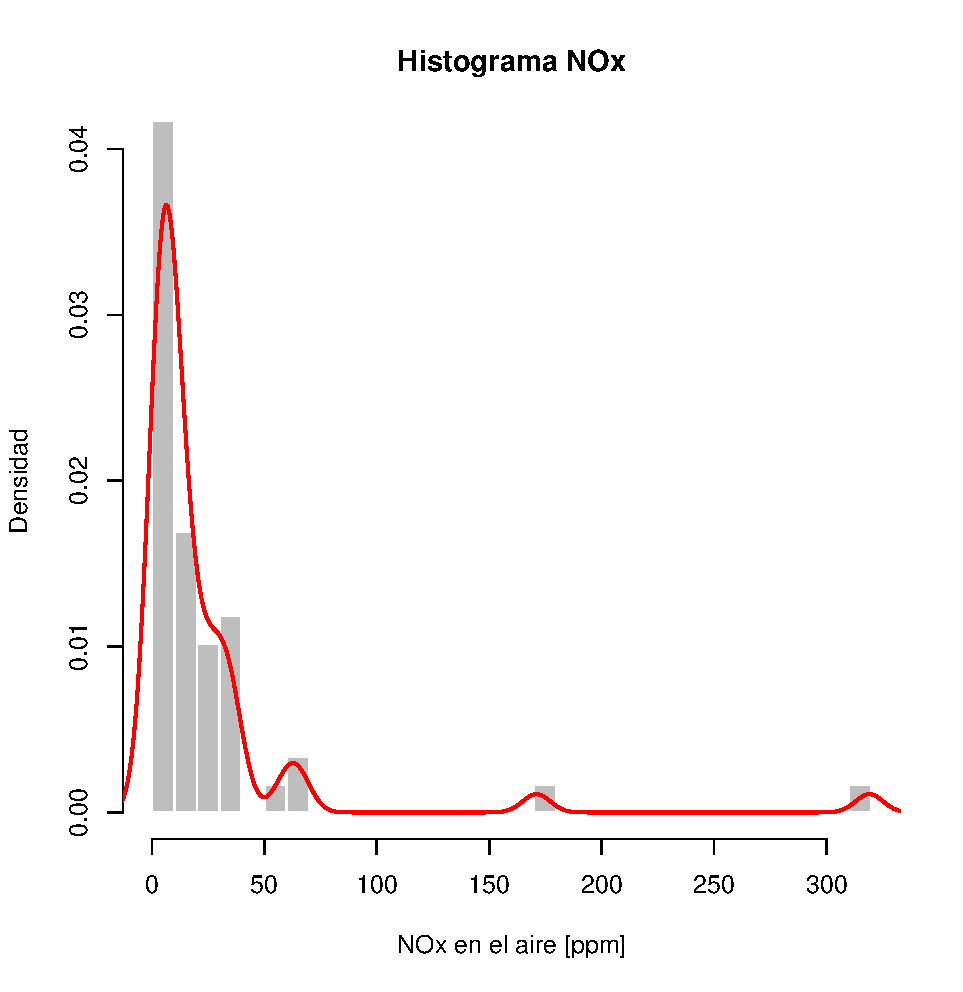
\includegraphics[width = 0.4\textwidth]{histnox}
\end{wrapfigure}

En el histograma de densidad, podemos observar todo lo que esperábamos. Un gráfico cargado a la izquierda, por esto la medida de skewness nos arrojó un valor positivo. Existe un par de valores que se escapan de la densidad general, justamente los que mencionamos en las medidas centrales. La mayoría de los datos se encuentran antes de los 50[ppm]. Podemos apreciar gráficamente la medida de kurtosis, en la punta del gráfico. 
\\
\\
\\
\\

\begin{wrapfigure}{l}{0.5\textwidth}
    \centering
    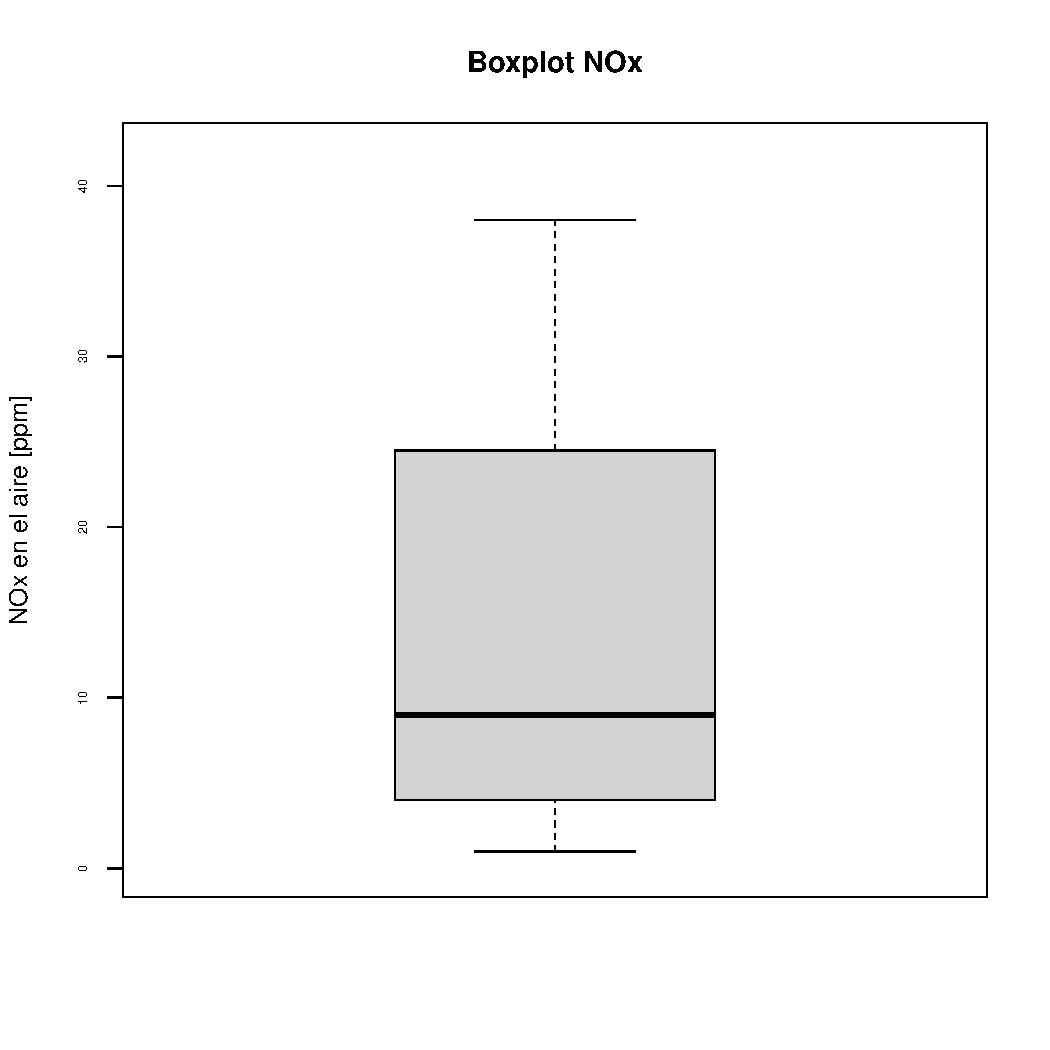
\includegraphics[width = 0.4\textwidth]{boxnox}
\end{wrapfigure}

Por último, el boxplot de los datos acota la mayor parte de su distribución antes de los 40[ppm]. Esto será algo a considerar más adelante cuando comparemos estos datos con otras variables. 

En definitiva, la variable de NOx si bien tiene algunos outliers, se concentra entre 1[ppm] y 40[ppm]
\\
\\
\\
\\
\\
\\

\subsubsection{HC}

\begin{center}
\begin{tabular}{|c|c|}
    \hline
    Variable & Unidad  \\ \hline
    HC & ppm \\
    \hline
\end{tabular}
\end{center}

\textbf{Medidas descriptivas de centro:}

\begin{center}
\begin{tabular}{|c|c|c|}
    \hline
    Promedio ponderado & Mediana & Moda \\ \hline
    38.4746 & 15 & 6 \\
    \hline
\end{tabular}
\end{center}

Al igual que los niveles de NOx, los niveles de HC en el aire presentan asimetría, juzgando los valores de medida central. De nuevo observamos que San Francisco (HC: 311[ppm]) y Los Ángeles-Long Beach (HC: 648[ppm]) se escapan bastante de los valores medios, y pueden ser considerados como outliers.
\\
\\
\textbf{Medidas descriptivas de posición:}

\begin{center}
\begin{tabular}{|c|c|c|c|c|}
    \hline
    Mínimo valor & Primer cuartil & Segundo cuartil & Tercer cuartil & Máximo valor\\ \hline
    1 & 7 & 15 & 30.5 & 648\\
    \hline
\end{tabular}
\end{center}

Comprobamos la idea anterior, el 75\% de los datos se encuentra antes de los 30.5[ppm].
\\
\\
\textbf{Medidas descriptivas de dispersión y forma:}

\begin{center}
\begin{tabular}{|c|c|c|c|c|}
    \hline
    Desviación estándar  & Varianza & Skewness & Kurtosis\\ \hline
    92.6388 & 8581.943 & 5.2732 & 30.0754\\
    \hline
\end{tabular}
\end{center}

Encontramos que las medidas de dispersión confirman nuestra hipótesis, esta variable tiene una dispersión y asimetría incluso mayor a la anterior, esto obviamente debido a que los valores que se escapan son incluso mayores a los que se escapan en la cantidad de NOx. La kurtosis es también mayor y por lo tanto de nuevo esperamos una forma puntiaguda en la línea de densidad.
\\
\\
\textbf{Gráficos de distribución:}
\\

\begin{wrapfigure}{r}{0.5\textwidth}
    \centering
    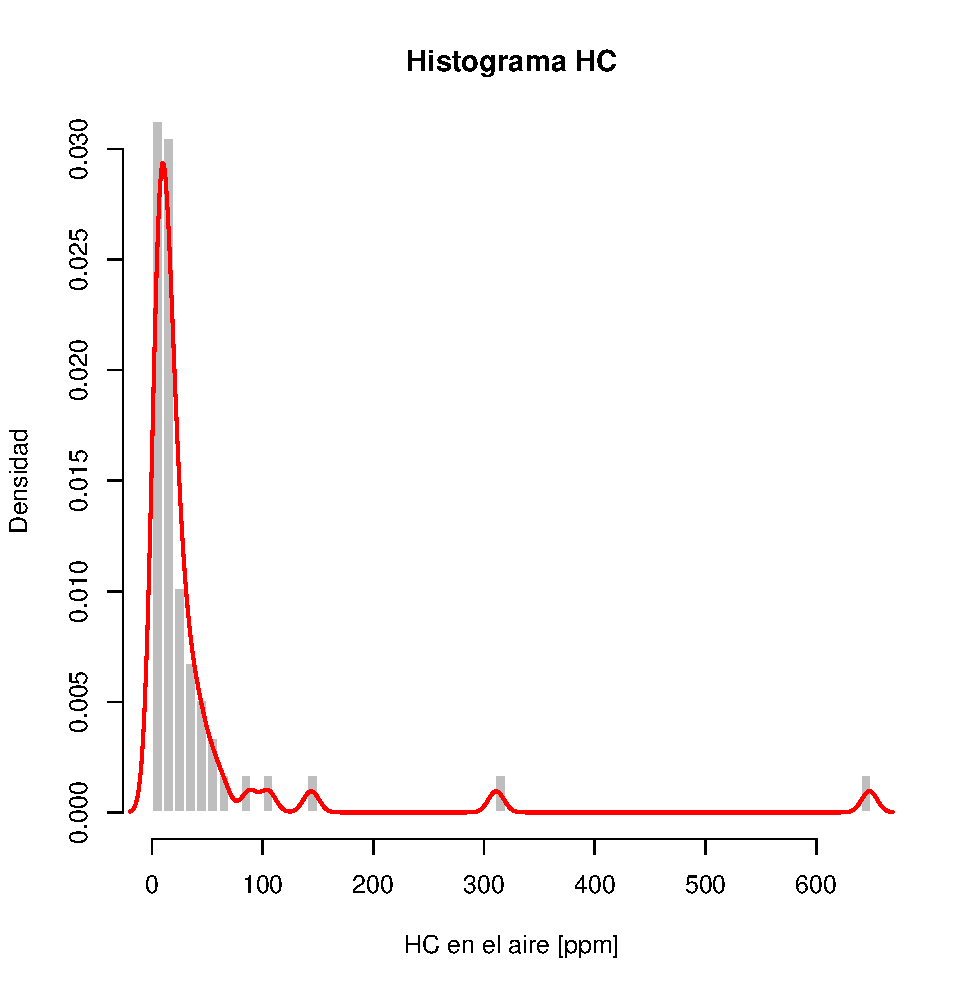
\includegraphics[width = 0.4\textwidth]{histhc}
\end{wrapfigure}

El histograma confirma el análisis anterior, muy cargado a la izquierda, puntiagudo y podemos observar los outliers de San Francisco y Los Ángeles-Long Beach. La mayoría de los datos se encuentran entre 1[ppm] y 100[ppm], esto se confirma al estudiar el boxplot de la variable.
\\
\\
\\
\\
\\
\\
\\
\\
\\
\\

\begin{wrapfigure}{l}{0.5\textwidth}
    \centering
    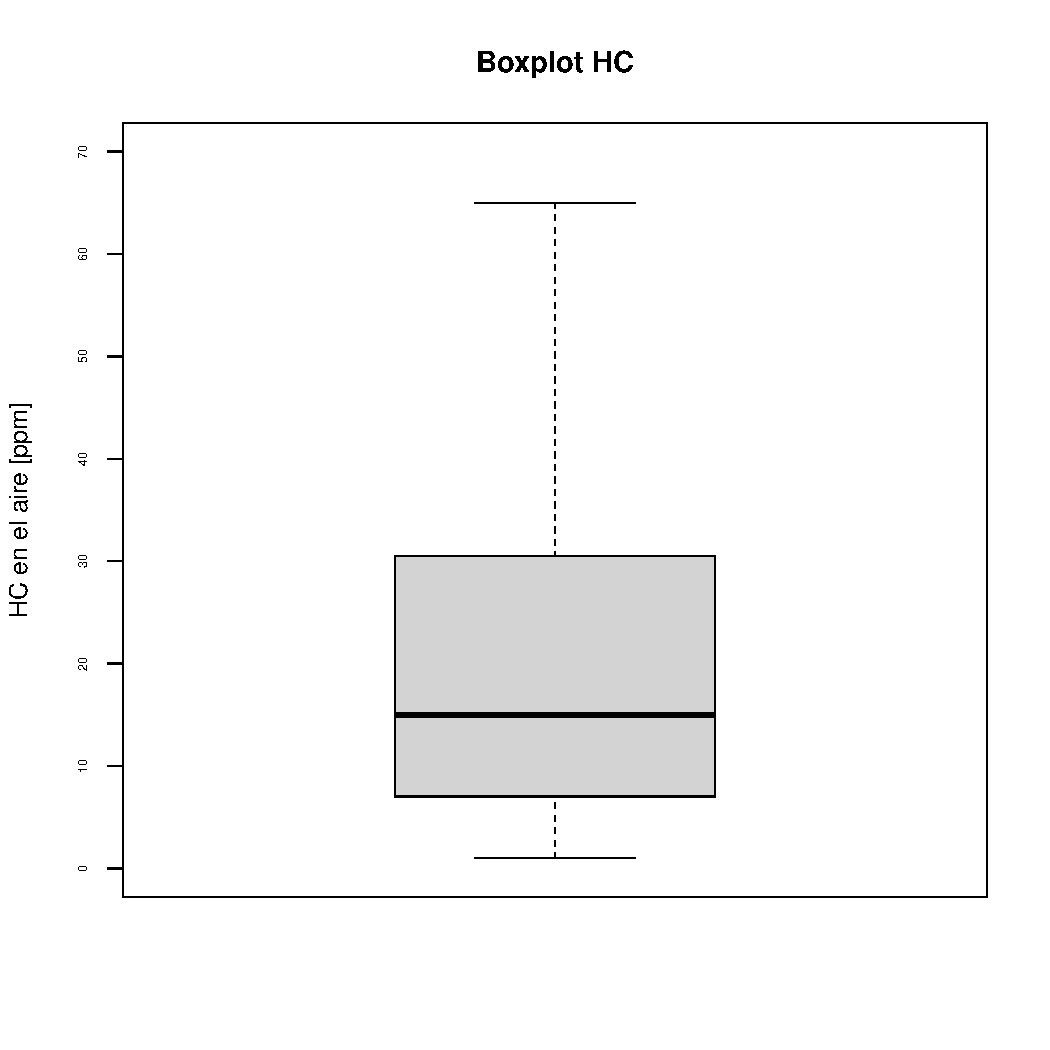
\includegraphics[width = 0.4\textwidth]{boxhc}
\end{wrapfigure}

En el boxplot de los datos, en el que no se muestran los outliers, la mayoría de mediciones se encuentra bajo los 70[ppm].

Con este análisis se desprende que la densidad de cantidades de HC se encuentra entre 1[ppm] y 70[ppm], esto debe considerarse al momento de relacionar la variable con otras, puesto que los outliers no entregan información estadísticamente concluyente.
\\
\\
\\
\\
\\
\subsubsection{SO_2}

\begin{center}
\begin{tabular}{|c|c|}
    \hline
    Variable & Unidad  \\ \hline
    SO_2 & ppm \\
    \hline
\end{tabular}
\end{center}

\textbf{Medidas descriptivas de centro:}

\begin{center}
\begin{tabular}{|c|c|c|}
    \hline
    Promedio ponderado & Mediana & Moda \\ \hline
    54.661 & 32 & 1 \\
    \hline
\end{tabular}
\end{center}

Como en los dos gases anteriores, se observa una gran diferencia entre las medidas descriptivas centrales de la variable SO_2.$ La moda es uno, por lo que este parece ser un gas menos común que los anteriores.
\\
\\
\textbf{Medidas descriptivas de posición:}

\begin{center}
\begin{tabular}{|c|c|c|c|c|}
    \hline
    Mínimo valor & Primer cuartil & Segundo cuartil & Tercer cuartil & Máximo valor\\ \hline
    1 & 13 & 32 & 70 & 278\\
    \hline
\end{tabular}
\end{center}

A pesar de las medidas de tendencia central, esta variable tiene una distribución más equitativa, según el estudio de sus cuartiles. También tiene un máximo menor al de los otros dos gases, confirmando que este aparece en menores cantidades
\\
\\
\textbf{Medidas descriptivas de dispersión y forma:}

\begin{center}
\begin{tabular}{|c|c|c|c|c|}
    \hline
    Desviación estándar  & Varianza & Skewness & Kurtosis\\ \hline
    63.5517 & 4038.814 & 1.8022 & 2.8894\\
    \hline
\end{tabular}
\end{center}

Las medidas de dispersión confirman que esta variable esta distribuida de manera más equitativa. Tiene, sin embargo, asimetría, otra vez inclinándose a la izquierda.La kurtosis es muho menor a las otras dos variables, lo que denota una concentración alrededor de la mediana también menor, un gráfico menos puntiagudo y más suave.
\\
\\
\textbf{Gráficos de distribución:}
\\

\begin{wrapfigure}{r}{0.5\textwidth}
    \centering
    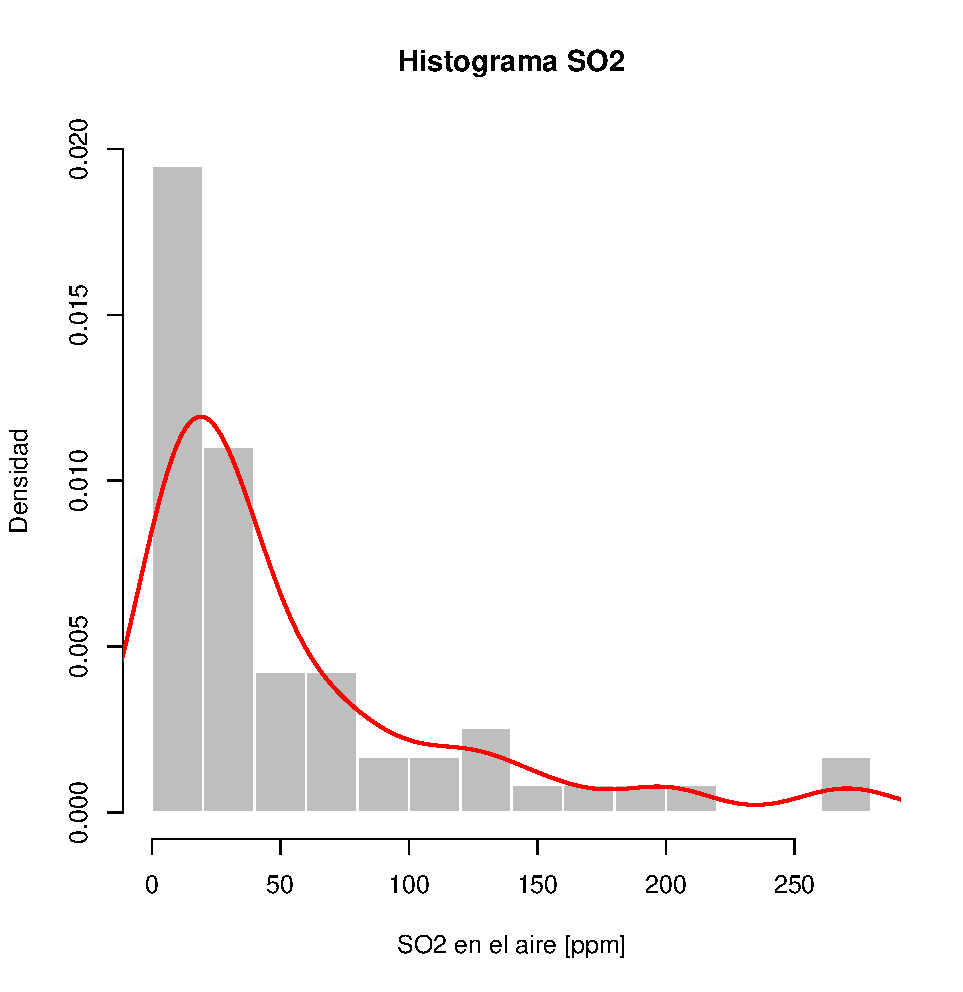
\includegraphics[width = 0.4\textwidth]{histso2}
\end{wrapfigure}

El histograma es, efectivamente, más equitativo. La kurtosis se nota menor pues la linea de densidad es mucho más suave que la de los otros dos gases. Si bien la medida de skewness resulto menor que en los otros dos, el gráfico parece estar igual de cargado a la izquierda. En realidad este valor fue menor porque el rango de valores de esta variable es menor, y los valores de la derecha son más comunes. La gran mayoría de los datos se encuentra antes de los 150[ppm].
\\
\\
\\
\\
\begin{wrapfigure}{l}{0.5\textwidth}
    \centering
    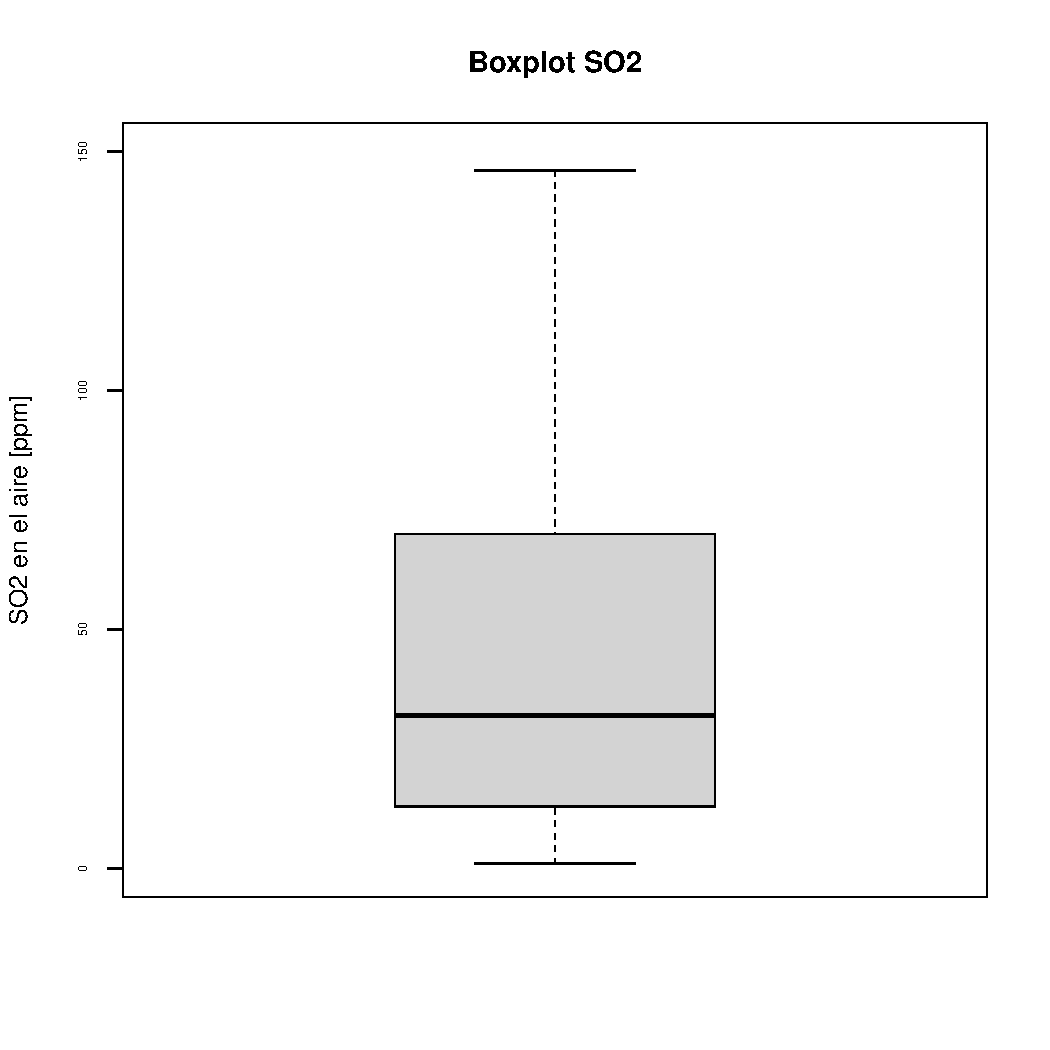
\includegraphics[width = 0.4\textwidth]{boxso2}
\end{wrapfigure}

Se confirma con el boxplot que la distribución de los valores tiene mayor densidad antes de los 150[ppm]

Las cantidades de SO_2$ son menores que las de los otros gases, y se acota su distribución más densa entre 1[ppm] y 150[ppm]. A pesar de lo anterior, los valores extremos no están tan alejados, así que de todas formas vale la pena observar su comportamiento.
\\
\\
\\
\\
\\

\subsection{Variables de población}

\subsubsection{Población total}

\begin{center}
\begin{tabular}{|c|c|}
    \hline
    Variable & Unidad  \\ \hline
    Población total & Número de personas \\
    \hline
\end{tabular}
\end{center}

\textbf{Medidas descriptivas de centro:}

\begin{center}
\begin{tabular}{|c|c|c|}
    \hline
    Promedio ponderado & Mediana & Moda \\ \hline
    1.438.037 & 914.427 & Ninguna \\
    \hline
\end{tabular}
\end{center}

Se observa una diferencia entre la esperanza y la mediana que indica asimetría en los datos. Al ser una variable de gran magnitud y valores muy específicos es dificil qe se produzca una moda, hay una probabilidad muy baja de que eligiendo 59 valores entre \sim$8.000.000 valores (diferencia entre el mínimo y máximo que se expone más adelante) uno se repita.
\\
\\
\textbf{Medidas descriptivas de posición:}

\begin{center}
\begin{tabular}{|c|c|c|c|c|}
    \hline
    Mínimo valor & Primer cuartil & Segundo cuartil & Tercer cuartil & Máximo valor\\ \hline
    124.833 & 566.515 & 914.427 & 1.717.201 & 8.274.961\\
    \hline
\end{tabular}
\end{center}

Vemos que, de nuevo, existe una tendencia a que aparezcan outliers mayores al dataset general, concentrándose la muestra en la porción que es menor a la media.
\\
\\
\textbf{Medidas descriptivas de dispersión y forma:}

\begin{center}
\begin{tabular}{|c|c|c|c|c|}
    \hline
    Desviación estándar  & Varianza & Skewness & Kurtosis\\ \hline
    1,54x10^6 & 2.38x10^8 & 2.7438 & 8.2747\\
    \hline
\end{tabular}
\end{center}

Si bien los valores de la desviación estándar y varianza son grandes, esto se debe en parte a la magnitud de la variable. La media de esta es ~1,48x10^6$, asi que un valor de esta magnitud nos indica una desviación mayor, pero dentro de lo esperable. La medida de skewness confirma que la muestra es más densa a la izquierda del gráfico, por último la kurtosis nos hace esperar una concentración mayor en la media y por lo tanto un gráfico ni tan suave ni tan puntiagudo.
\\
\\
\textbf{Gráficos de distribución:}
\\

\begin{wrapfigure}{r}{0.5\textwidth}
    \centering
    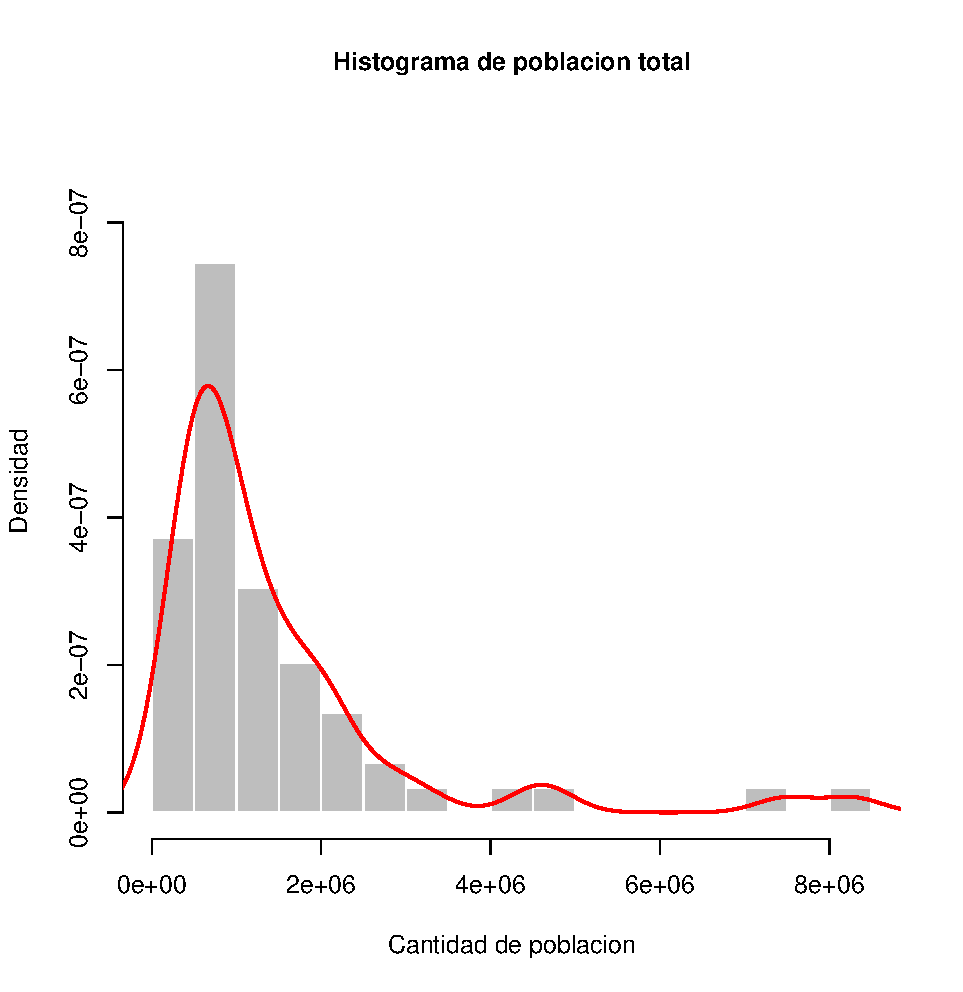
\includegraphics[width = 0.4\textwidth]{histpt}
\end{wrapfigure}

El histograma, como esperábamos, está cargado a la izquierda. Podemos ver los outliers y que la mayor parte de los datos se encuentra antes de 2x10^6$. Se observa la punta que sugería la kurtosis. 
\\
\\
\\
\\
\\
\\
\\
\\
\\
\\
\\
\begin{wrapfigure}{l}{0.5\textwidth}
    \centering
    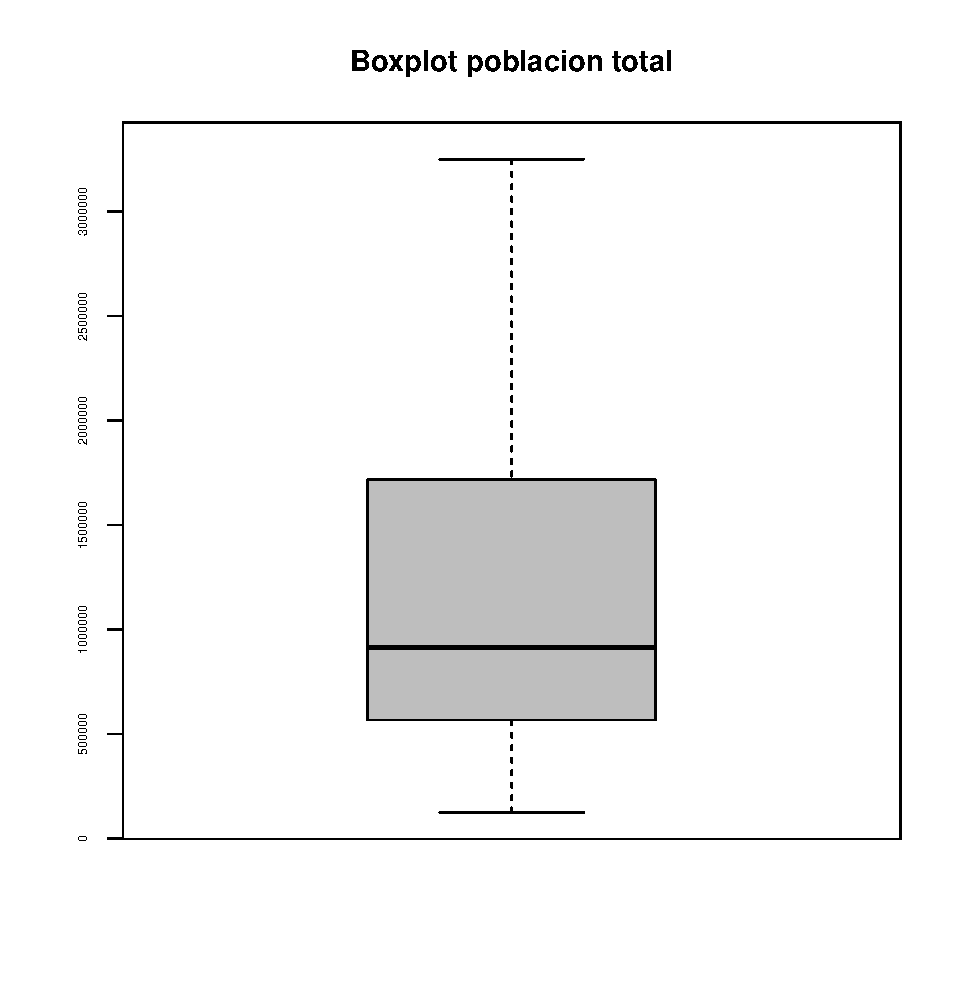
\includegraphics[width = 0.4\textwidth]{boxpt}
\end{wrapfigure}

Por último el boxplot muestra que los datos se concentran bajo los 3.000.000, mostrando una densidad muy cargada alrededor del millón de personas. Los datos corresponden a ciudades grandes pero no masivas (exceptuando los outliers). Como punto de referencia Santiago tiene alrededor de 5 millones de personas (datos no tan confiables dado nuestro último censo).
\\
\\
\\
\\
\\
\\

\subsubsection{Población por hogar}

\begin{center}
\begin{tabular}{|c|c|}
    \hline
    Variable & Unidad  \\ \hline
    Población por hogar & Número de personas \\
    \hline
\end{tabular}
\end{center}

Esta variable es un promedio de la cantidad de personas que viven en un domicilio particular para cada ciudad.
\\

\textbf{Medidas descriptivas de centro:}

\begin{center}
\begin{tabular}{|c|c|c|}
    \hline
    Promedio ponderado & Mediana & Moda \\ \hline
    3.2466 & 3.27 & 3.21 y 3.32 \\
    \hline
\end{tabular}
\end{center}

Las medidas de tendencia central de esta variable son muy cercanas, por lo que esperamos simetría. Era de esperar este resultado pues en nuestra cultura occidental el número de personas en cada casa no varía mucho más allá del rango 1-6.
\\
\\
\textbf{Medidas descriptivas de posición:}

\begin{center}
\begin{tabular}{|c|c|c|c|c|}
    \hline
    Mínimo valor & Primer cuartil & Segundo cuartil & Tercer cuartil & Máximo valor\\ \hline
    2.65 & 3.21 & 3.27 & 3.36 & 3.53\\
    \hline
\end{tabular}
\end{center}

A pesar de la simetría que sugieren las medidas de tendencia central, vemos que el valor mínimo se escapa más de la media de lo que lo hace el valor máximo, lo que sugiere que los datos están un poco cargados a la derecha.
\\
\\
\textbf{Medidas descriptivas de dispersión y forma:}

\begin{center}
\begin{tabular}{|c|c|c|c|c|}
    \hline
    Desviación estándar  & Varianza & Skewness & Kurtosis\\ \hline
    0.1829 & 0.0335 & -1.6032 & 3.1184\\
    \hline
\end{tabular}
\end{center}

La desviación estándar es pequeña, lo que era de esperarse por la magnitud de diferencia entre los valores y por la distribución simétrica de estos. El skewness confirma que el gráfico está un poco cargado a la derecha y la kurtosis nos hace esperar una forma más bien suave.
\\
\\
\\
\\
\\
\\
\\
\\
\\
\\
\\
\\
\\
\textbf{Gráficos de distribución:}
\\

\begin{wrapfigure}{r}{0.5\textwidth}
    \centering
    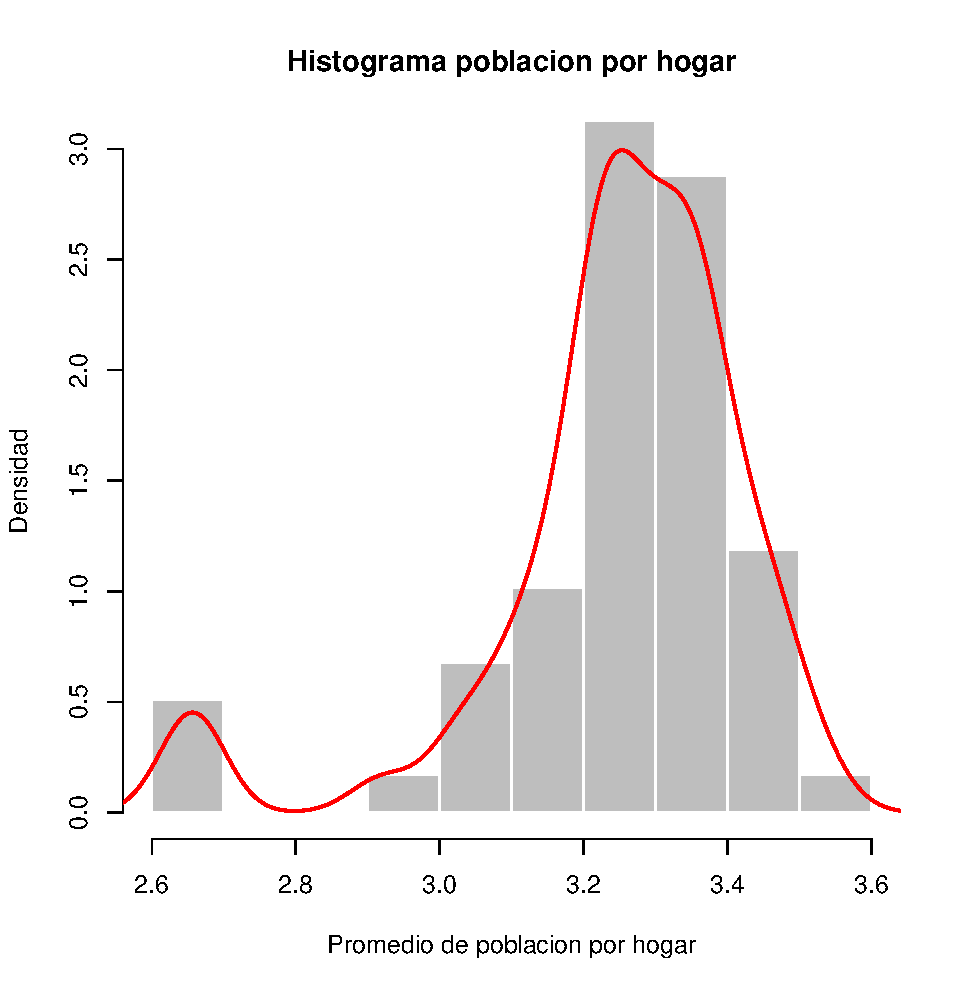
\includegraphics[width = 0.4\textwidth]{histph}
\end{wrapfigure}

El histograma efectivamente está cargado a la derecha, pero podemos observar que esto se debe a un outlier ubicado a la izquierda. Sin este, la distribución sería muy simétrica, y es por esto que los valores de medida central son tan cercanos. La forma es suave, como predijo la kurtosis y parece tener dos puntas, probablemente causado por la naturaleza multimodal de la variable.
\\
\\
\\
\\
\\
\begin{wrapfigure}{l}{0.5\textwidth}
    \centering
    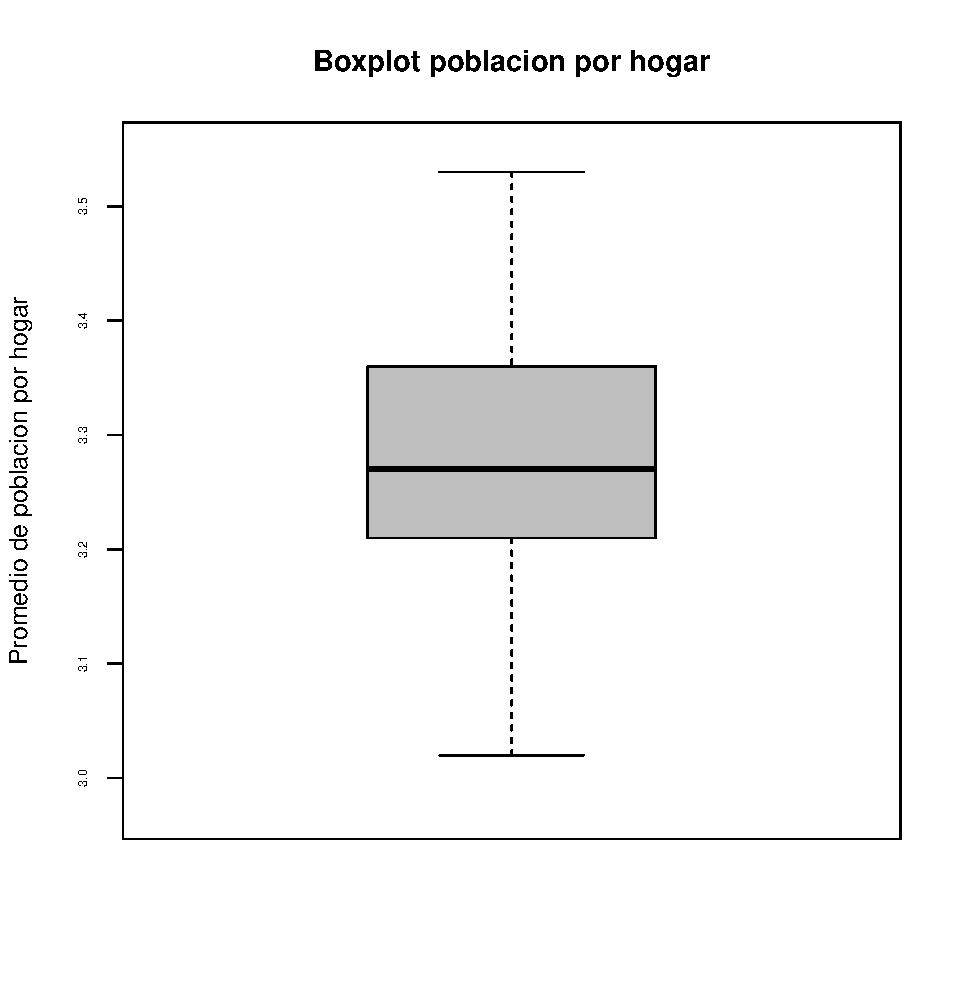
\includegraphics[width = 0.4\textwidth]{boxph}
\end{wrapfigure}

El boxplot, que deja afuera al outlier, presenta la simetría esperada.
\\
\\
\\
\\
\\
\\
\\
\\
\\
\\
\\
\\
\\
\\
\subsubsection{Ingresos medios}

\begin{center}
\begin{tabular}{|c|c|}
    \hline
    Variable & Unidad  \\ \hline
    Ingresos medios anuales & Miles de USD \\
    \hline
\end{tabular}
\end{center}
\\
\\

\textbf{Medidas descriptivas de centro:}

\begin{center}
\begin{tabular}{|c|c|c|}
    \hline
    Promedio ponderado & Mediana & Moda \\ \hline
    33246.66 & 32452 & Ninguna \\
    \hline
\end{tabular}
\end{center}

Al igual que en la variable de población total, es difícil que se presentara una moda. Las otras dos medidas son cercanas asi que debiese existir simetría en los datos.
\\
\\
\textbf{Medidas descriptivas de posición:}

\begin{center}
\begin{tabular}{|c|c|c|c|c|}
    \hline
    Mínimo valor & Primer cuartil & Segundo cuartil & Tercer cuartil & Máximo valor\\ \hline
    25782 & 30004.5 & 32452 & 35496 & 47966\\
    \hline
\end{tabular}
\end{center}

La distribución presenta una naturaleza simétrica, concentrándose los datos entre el primer y tercer cuartil, y los extremos están separados equitativamente.
\\
\\
\textbf{Medidas descriptivas de dispersión y forma:}

\begin{center}
\begin{tabular}{|c|c|c|c|c|}
    \hline
    Desviación estándar  & Varianza & Skewness & Kurtosis\\ \hline
    4.47x10^3 & 2x10^7 & 1.2131 & 1.6983\\
    \hline
\end{tabular}
\end{center}

La desviación estándar no es tanta (magnitud 10^3$ en una variable de magnitud 10^4$) pero muestra que los datos están distribuidos, por lo mismo la kurtosis es pequeña. El skewness es tampoco es muy elevado pero de todas formas existe una inclinación de los datos hacia la izquierda.
\\
\\
\textbf{Gráficos de distribución:}
\\

\begin{wrapfigure}{r}{0.5\textwidth}
    \centering
    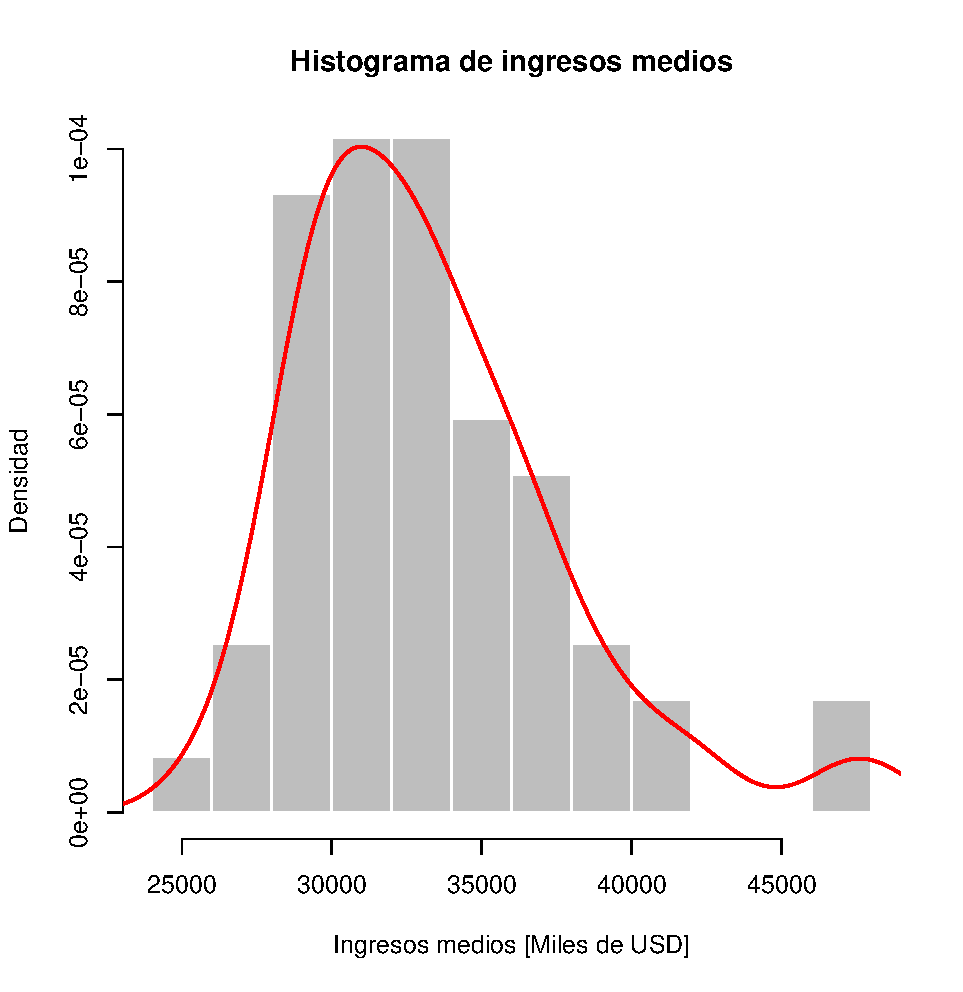
\includegraphics[width = 0.4\textwidth]{histim}
\end{wrapfigure}

Hay un outlier a la  derecha que es el que 'arruina' la simetría de los datos, de todas maneras la parte densa de estos se inclina un poco a la izquierda. La kurtosis define esa forma suave.
\\
\\
\\
\\
\\
\\
\\
\\
\\
\\
\\
\begin{wrapfigure}{l}{0.5\textwidth}
    \centering
    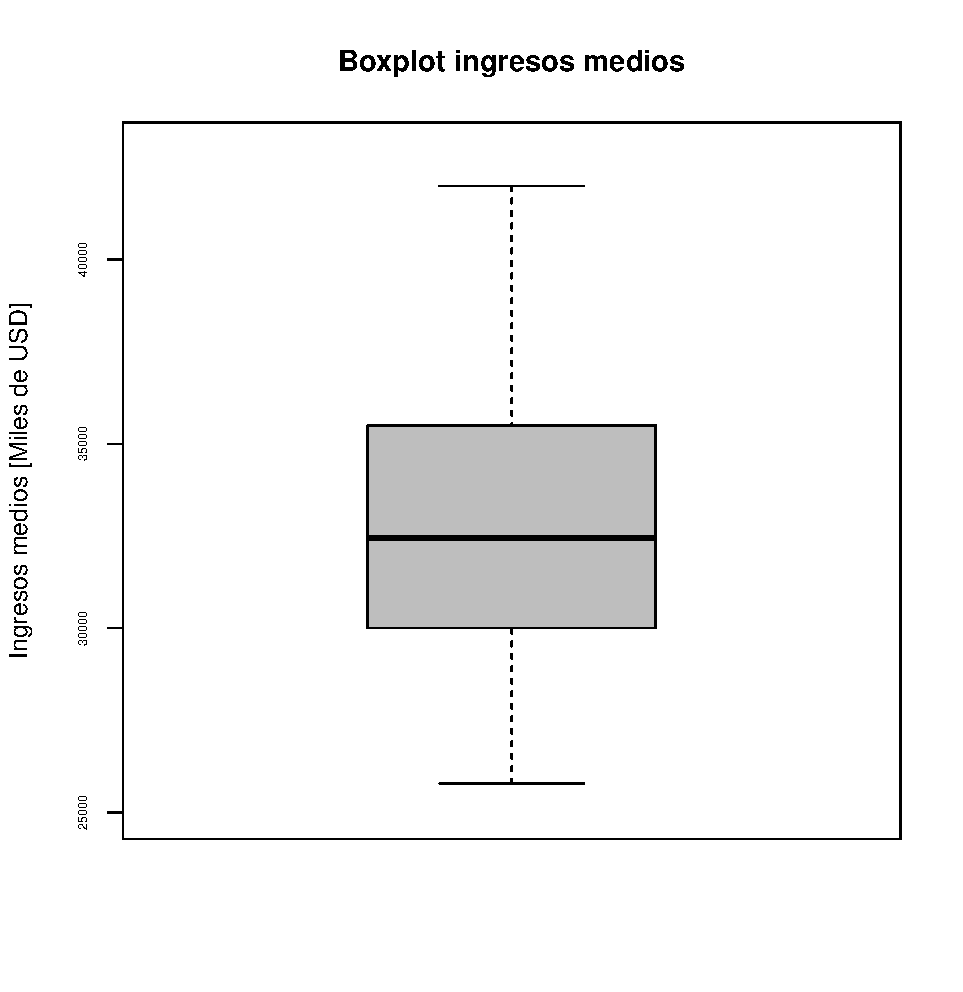
\includegraphics[width = 0.4\textwidth]{boxim}
\end{wrapfigure}

El boxplot es simétrico, con tendencia a la baja.
\\
\\
\\
\\
\\
\\
\\
\\
\\
\\
\\
\\
\\
\\

\subsubsection{Mortalidad}

\begin{center}
\begin{tabular}{|c|c|}
    \hline
    Variable & Unidad  \\ \hline
    Mortalidad (por mil habitantes) & Cantidad de personas \\
    \hline
\end{tabular}
\end{center}
\\
\\

\textbf{Medidas descriptivas de centro:}

\begin{center}
\begin{tabular}{|c|c|c|}
    \hline
    Promedio ponderado & Mediana & Moda \\ \hline
    941.1731 & 946.19 & Ninguna \\
    \hline
\end{tabular}
\end{center}

La mortalidad parece ser simétrica, la mediana y media son cercanas sobre todo considerando la magnitud de la variable.
\\
\\
\textbf{Medidas descriptivas de posición:}

\begin{center}
\begin{tabular}{|c|c|c|c|c|}
    \hline
    Mínimo valor & Primer cuartil & Segundo cuartil & Tercer cuartil & Máximo valor\\ \hline
    790.73 & 899.395 & 946.19 & 984.12 & 1113.16\\
    \hline
\end{tabular}
\end{center}

La distribución presenta una naturaleza simétrica, concentrándose los datos entre el primer y tercer cuartil, y los extremos están separados equitativamente.
\\
\\
\textbf{Medidas descriptivas de dispersión y forma:}

\begin{center}
\begin{tabular}{|c|c|c|c|c|}
    \hline
    Desviación estándar  & Varianza & Skewness & Kurtosis\\ \hline
    62.4213 & 3896.423 & 0.0629 & -0.0495\\
    \hline
\end{tabular}
\end{center}

La desviación estándar es mediana, por lo que los datos están distribuidos a lo largo del soporte. El skewness es muy bajo por lo que esperamos bastante simetría. La kurtosis es negativa así que el gráfico es mas bien suave, platicúrtico.
\\
\\
\textbf{Gráficos de distribución:}
\\

\begin{wrapfigure}{r}{0.5\textwidth}
    \centering
    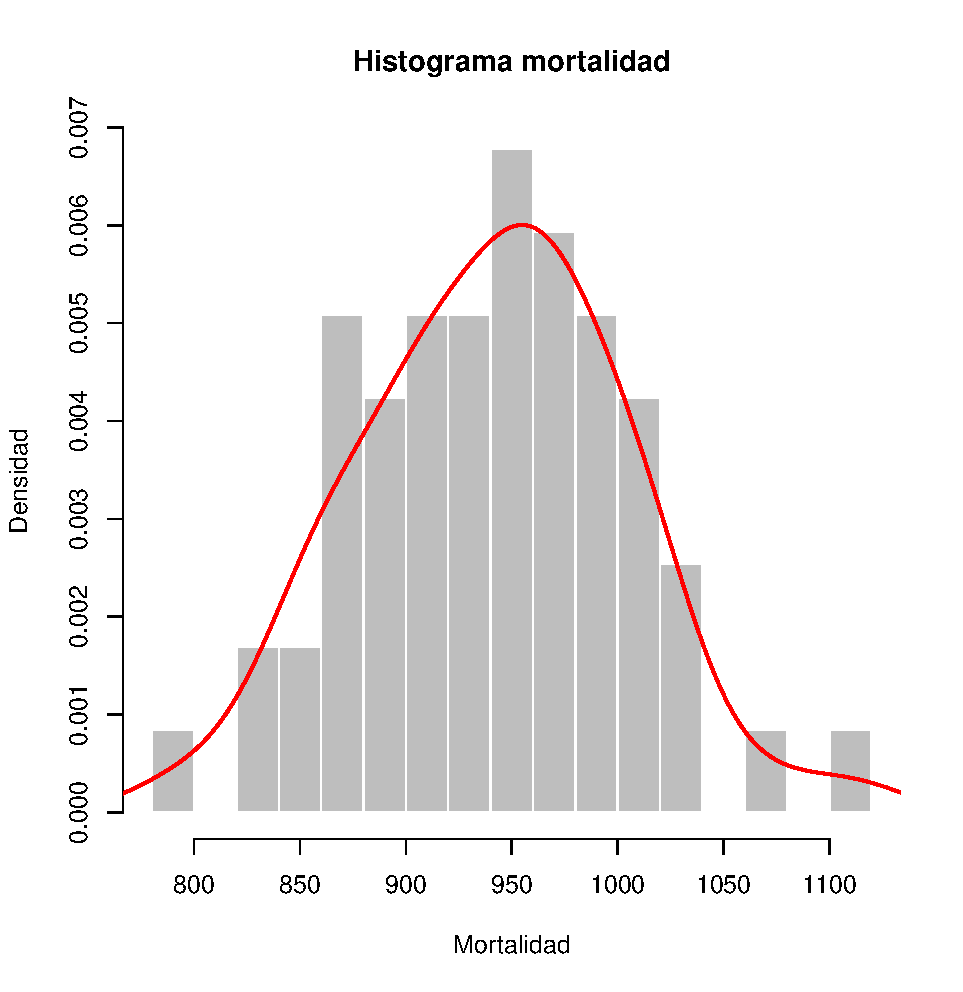
\includegraphics[width = 0.4\textwidth]{histmo}
\end{wrapfigure}

Como se puede apreciar en el histograma, la variable presenta una naturaleza simétrica.
\\
\\
\\
\\
\\
\\
\\
\\
\\
\\
\\
\\
\\
\begin{wrapfigure}{l}{0.5\textwidth}
    \centering
    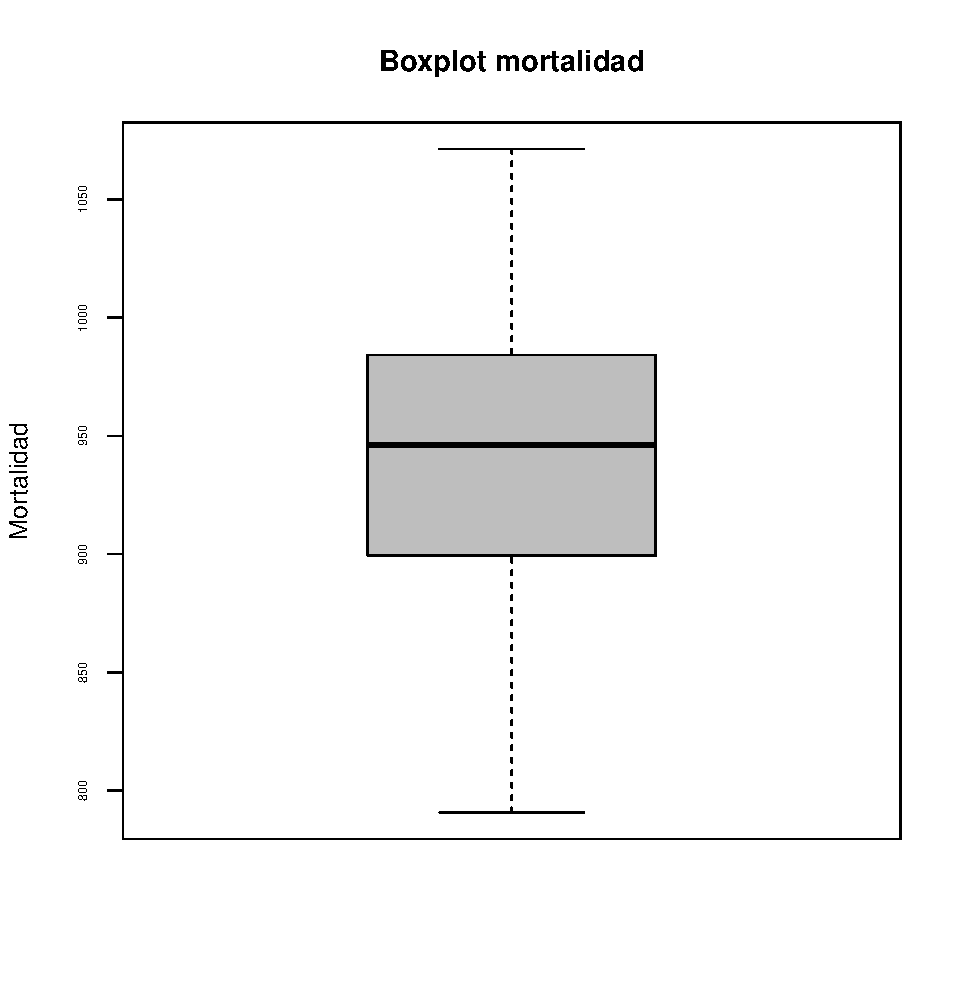
\includegraphics[width = 0.4\textwidth]{boxmo}
\end{wrapfigure}

El boxplot es simétrico, con tendencia a la alza. Abarca la mayoría de los datos.
\\
\\
\\
\\
\\
\\
\\
\\
\\
\\
\\
\\
\\

\subsection{Variables mediambientales}

\subsubsection{Cantidad de lluvia}

\begin{center}
\begin{tabular}{|c|c|}
    \hline
    Variable & Unidad  \\ \hline
    Lluvia caída & Pulgadas \\
    \hline
\end{tabular}
\end{center}
\\
\\

\textbf{Medidas descriptivas de centro:}

\begin{center}
\begin{tabular}{|c|c|c|}
    \hline
    Promedio ponderado & Mediana & Moda \\ \hline
    38.5085  & 38 & 36, 35 y 42 \\
    \hline
\end{tabular}
\end{center}

Esta es una variable multimodal, esto puede deberse a que algunas ciudades son cercanas. Se denota una cercanía entre los valores que hace pensar en simetría de la variable.
\\
\\
\textbf{Medidas descriptivas de posición:}

\begin{center}
\begin{tabular}{|c|c|c|c|c|}
    \hline
    Mínimo valor & Primer cuartil & Segundo cuartil & Tercer cuartil & Máximo valor\\ \hline
    10 & 33.5 & 38 & 44 & 65\\
    \hline
\end{tabular}
\end{center}

La distribución presenta una naturaleza simétrica, concentrándose los datos entre el primer y tercer cuartil, y los extremos están bastante separados (con respecto al centro) por lo que podemos esperar que la línea de densidad tenga colas más largas.
\\
\\
\textbf{Medidas descriptivas de dispersión y forma:}

\begin{center}
\begin{tabular}{|c|c|c|c|c|}
    \hline
    Desviación estándar  & Varianza & Skewness & Kurtosis\\ \hline
    11.57 & 133.94 & -0.1724 & 0.6749\\
    \hline
\end{tabular}
\end{center}

La desviación estándar es considerable, lo que reafirma la idea de datos más dispersos y no tan concentrados, por eso la kurtosis es tan pequeña. El skewness es bajo también lo que denota simetría.
\\
\\
\textbf{Gráficos de distribución:}
\\

\begin{center}
    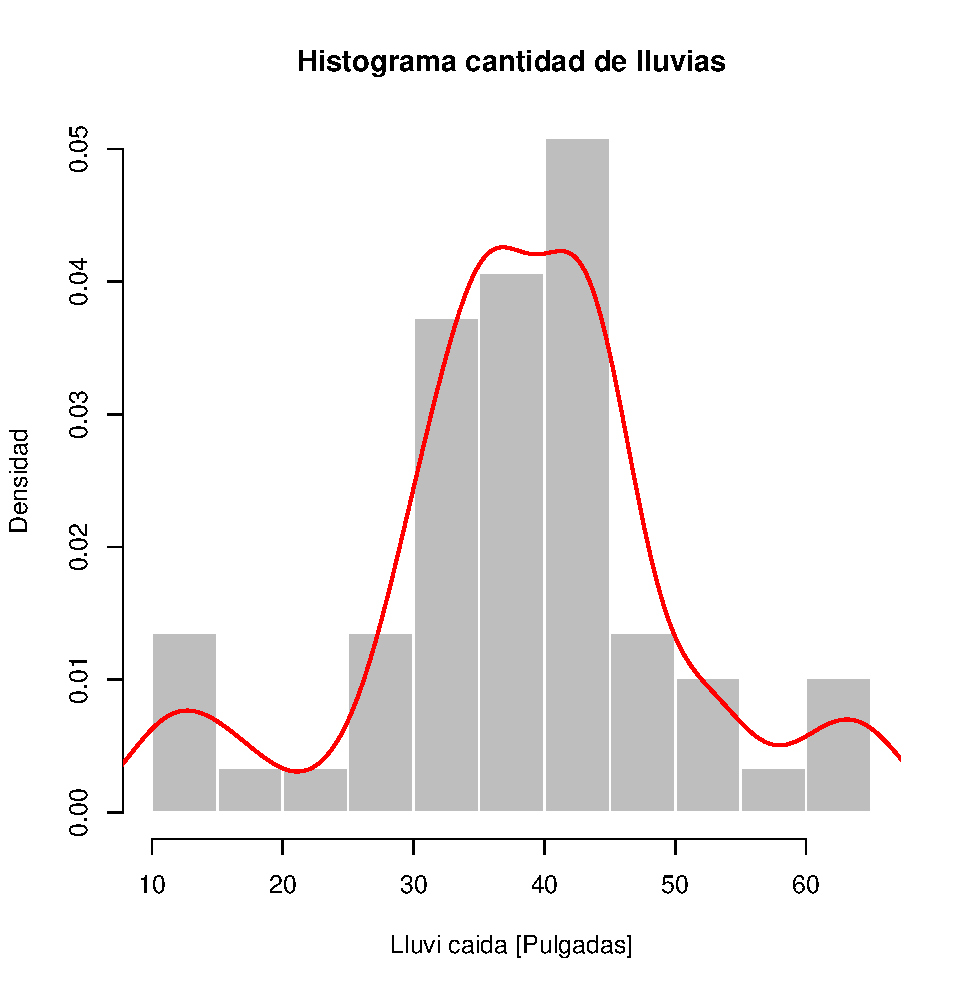
\includegraphics[scale = 0.3]{histll}
    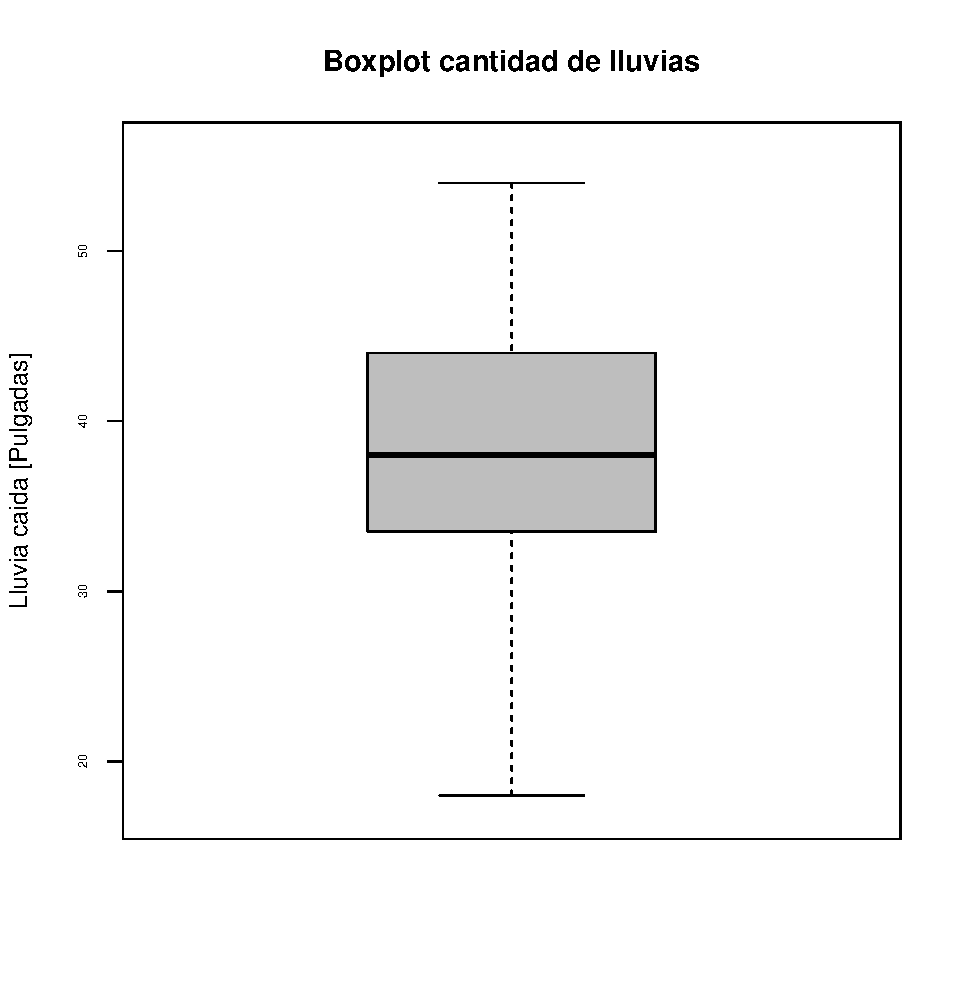
\includegraphics[scale = 0.3]{boxll}
\end{center}

Se puede apreciar la simetría del histograma y del boxplot, aunque este último tiene una tendencia al alza que se observa también en las barras. Es esta pequeña asimetría la que nos entrega ese valor de skewness negativo. La doble punta probablemente se deba a la naturaleza multimodal.

\subsubsection{Humedad}

\begin{center}
\begin{tabular}{|c|c|}
    \hline
    Variable & Unidad  \\ \hline
    Humedad & Porcentaje de humedad en el aire \\
    \hline
\end{tabular}
\end{center}
\\
\\

\textbf{Medidas descriptivas de centro:}

\begin{center}
\begin{tabular}{|c|c|c|}
    \hline
    Promedio ponderado & Mediana & Moda \\ \hline
    57.7458  & 57 & 56 \\
    \hline
\end{tabular}
\end{center}

Esta variable presenta simetría.
\\
\\
\textbf{Medidas descriptivas de posición:}

\begin{center}
\begin{tabular}{|c|c|c|c|c|}
    \hline
    Mínimo valor & Primer cuartil & Segundo cuartil & Tercer cuartil & Máximo valor\\ \hline
    38 & 55.5 & 57 & 60 & 73\\
    \hline
\end{tabular}
\end{center}

Se presenta una mayor concentración alrededor de la mediana y una pequeña tendencia hacia los valores menores.
\\
\\
\textbf{Medidas descriptivas de dispersión y forma:}

\begin{center}
\begin{tabular}{|c|c|c|c|c|}
    \hline
    Desviación estándar  & Varianza & Skewness & Kurtosis\\ \hline
    5.38 & 28.95 & 0.1959 & 3.652\\
    \hline
\end{tabular}
\end{center}

La desviación estándar es mediana. El skewness confirma que los datos están un poco cargados a la izquerda y la kurtosis se debe a la densidad de datos en el medio del soporte.
\\
\\
\textbf{Gráficos de distribución:}
\\

\begin{center}
    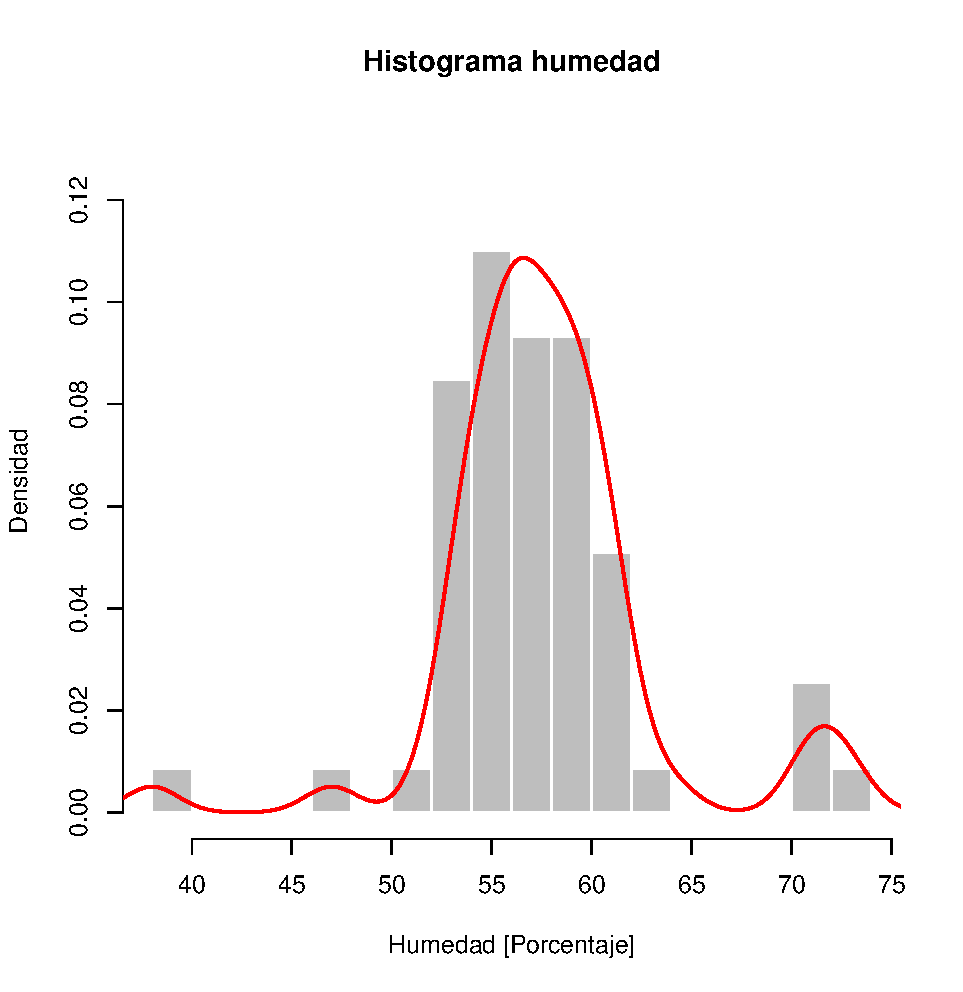
\includegraphics[scale = 0.3]{histhu}
    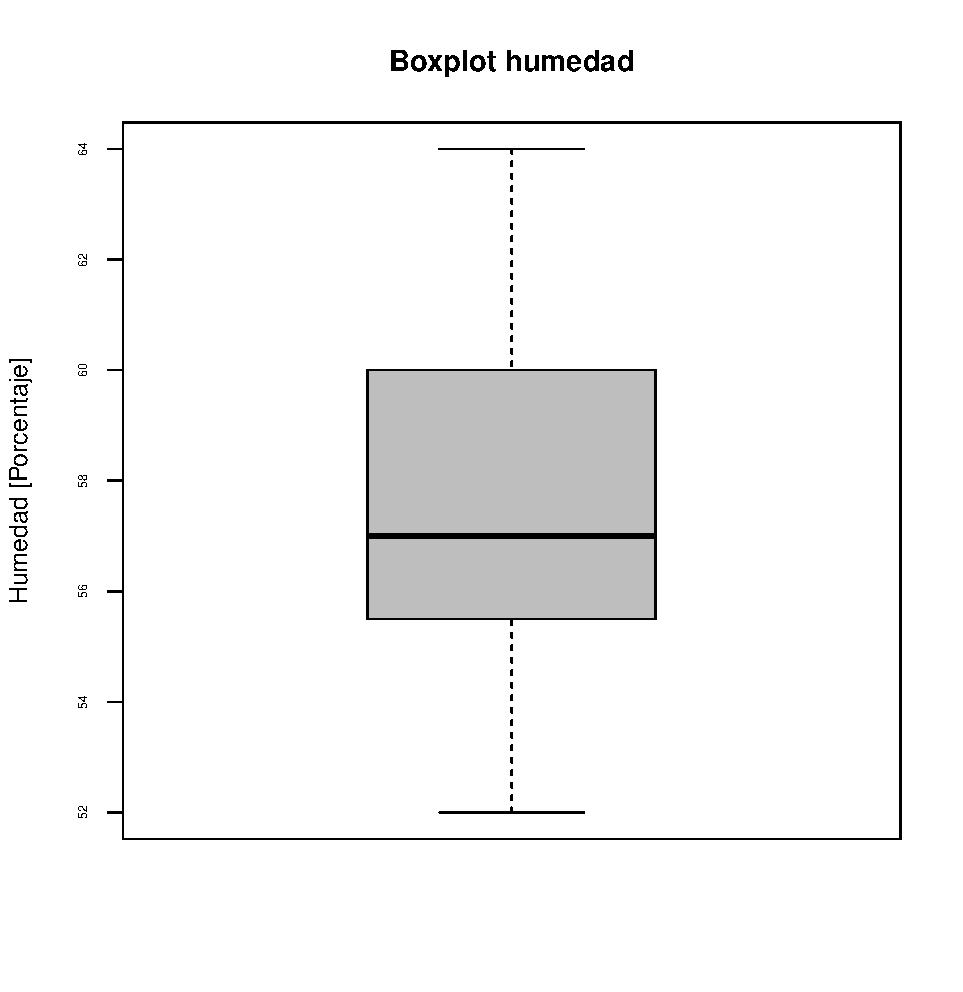
\includegraphics[scale = 0.3]{boxhu}
\end{center}

Podemos observar claramente en el histograma que la mayor densidad de datos se concentra en el medio, por esto la punta que sugiere la kurtosis. El boxplot nos muestra la tendencia a la baja que esperábamos por el valor del skewness.

\subsubsection{Temperaturas en Enero}

\begin{center}
\begin{tabular}{|c|c|}
    \hline
    Variable & Unidad  \\ \hline
    Temperatura en el mes de Enero & Fahrenheit \\
    \hline
\end{tabular}
\end{center}
\\
Se presenta el promedio de las temperaturas registradas en el mes de Enero.
\\

\textbf{Medidas descriptivas de centro:}

\begin{center}
\begin{tabular}{|c|c|c|}
    \hline
    Promedio ponderado & Mediana & Moda \\ \hline
    33.7966  & 31 & 30 y 24 \\
    \hline
\end{tabular}
\end{center}

Es una variable multimodal, que presenta una pequeña tendencia hacia los valores menores.
\\
\\
\textbf{Medidas descriptivas de posición:}

\begin{center}
\begin{tabular}{|c|c|c|c|c|}
    \hline
    Mínimo valor & Primer cuartil & Segundo cuartil & Tercer cuartil & Máximo valor\\ \hline
    12 & 27 & 31 & 39.5 & 67\\
    \hline
\end{tabular}
\end{center}

Confirmamos que los datos se cargan hacia la izquierda, con un máximo que probablemente sea considerado como outlier.
\\
\\
\textbf{Medidas descriptivas de dispersión y forma:}

\begin{center}
\begin{tabular}{|c|c|c|c|c|}
    \hline
    Desviación estándar  & Varianza & Skewness & Kurtosis\\ \hline
    10.15 & 103.06 & 0.9659 & 0.9072\\
    \hline
\end{tabular}
\end{center}

La desviación estándar es mediana. El skewness y la kurtosis son bajos, la variable es bastante simétrica con una inclinación hacia la izquierda y debiese tener forma suave.
\\
\\
\textbf{Gráficos de distribución:}
\\

\begin{center}
    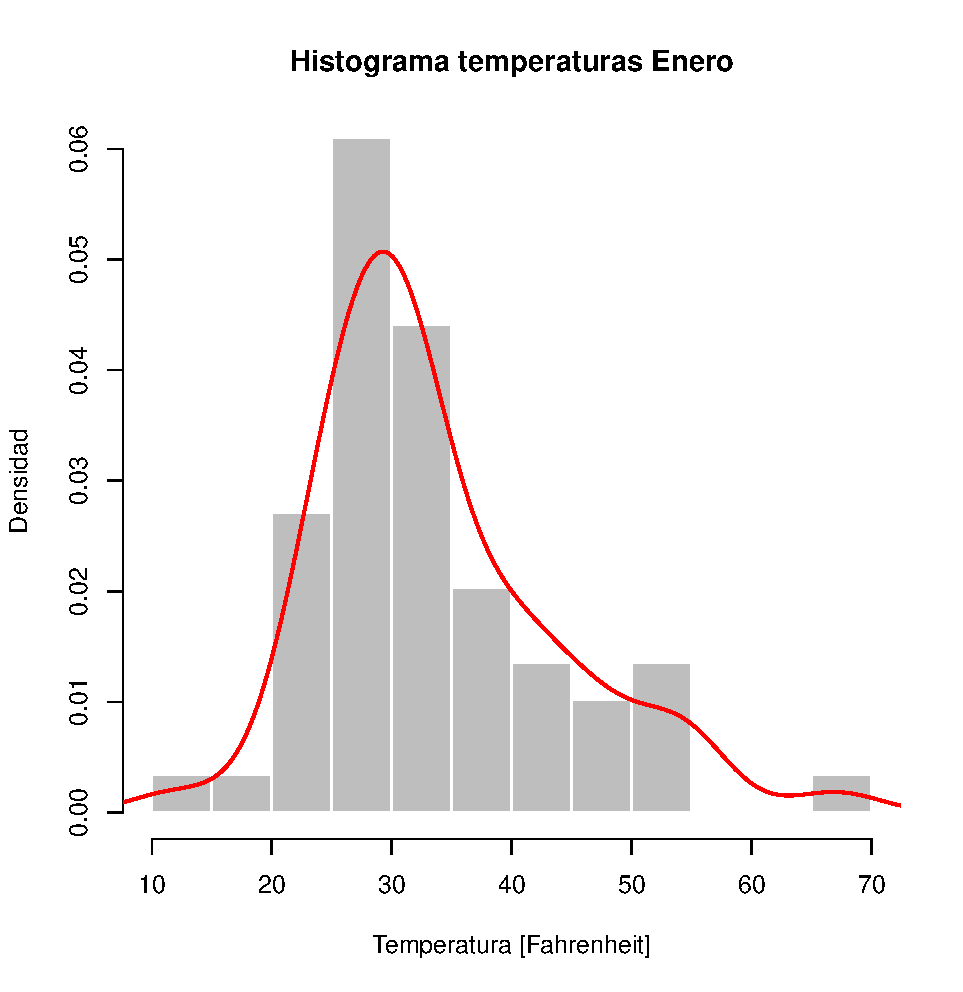
\includegraphics[scale = 0.3]{histte}
    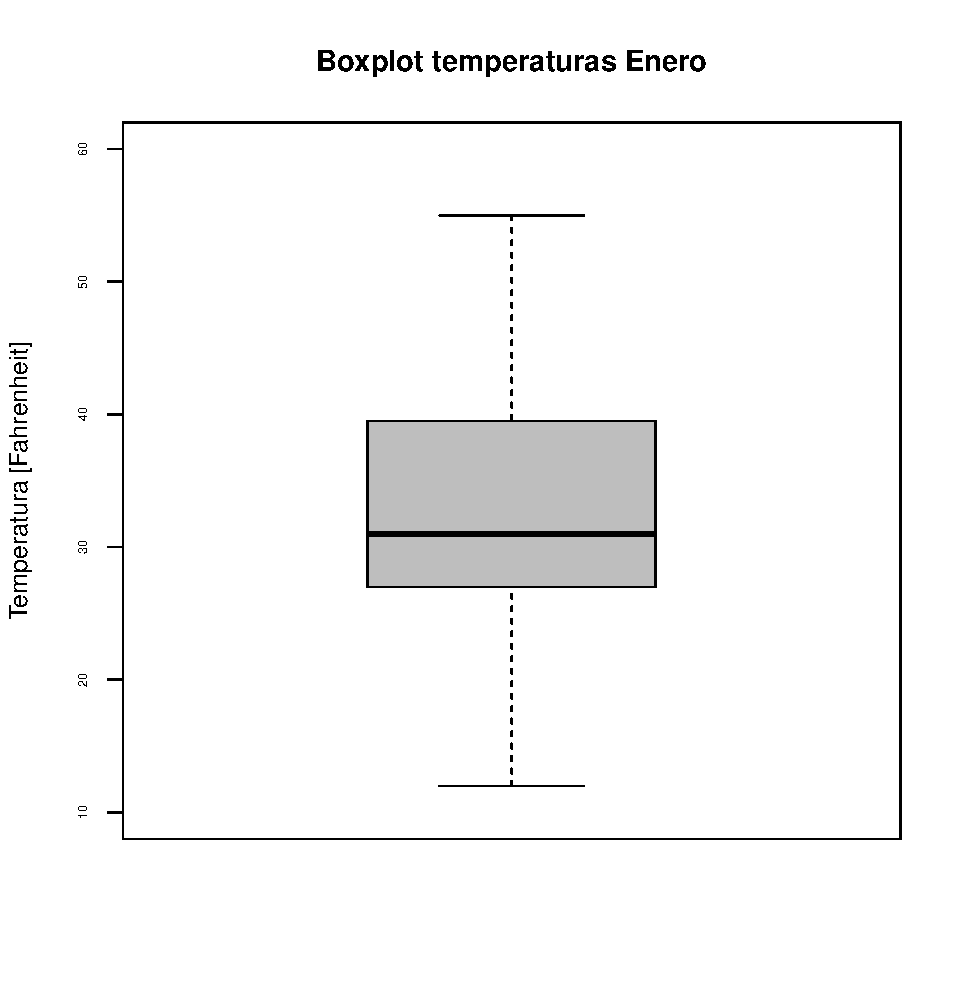
\includegraphics[scale = 0.3]{boxte}
\end{center}

En los gráficos se observa claramente el analisis anterior, se ve la inclinación, el outlier y la forma relativamente suave.

\subsubsection{Temperaturas en Julio}

\begin{center}
\begin{tabular}{|c|c|}
    \hline
    Variable & Unidad  \\ \hline
    Temperatura en el mes de Julio & Fahrenheit \\
    \hline
\end{tabular}
\end{center}
\\
Se presenta el promedio de las temperaturas registradas en el mes de Julio.
\\

\textbf{Medidas descriptivas de centro:}

\begin{center}
\begin{tabular}{|c|c|c|}
    \hline
    Promedio ponderado & Mediana & Moda \\ \hline
    74.4  & 74 & 72 \\
    \hline
\end{tabular}
\end{center}

Variable simétrica, con una pequeña tendencia a la baja.
\\
\\
\textbf{Medidas descriptivas de posición:}

\begin{center}
\begin{tabular}{|c|c|c|c|c|}
    \hline
    Mínimo valor & Primer cuartil & Segundo cuartil & Tercer cuartil & Máximo valor\\ \hline
    63 & 72 & 74 & 77 & 85\\
    \hline
\end{tabular}
\end{center}

Confirmamos que los datos se cargan hacia la izquierda, con extremos equitativamente distribuidas.
\\
\\
\textbf{Medidas descriptivas de dispersión y forma:}

\begin{center}
\begin{tabular}{|c|c|c|c|c|}
    \hline
    Desviación estándar  & Varianza & Skewness & Kurtosis\\ \hline
    4.6 & 21.18 & 0.0632 & -0.1576\\
    \hline
\end{tabular}
\end{center}

La desviación estándar es pequeña. El skewness y la kurtosis son bajos, la variable es bastante simétrica y debiese tener forma suave.
\\
\\
\textbf{Gráficos de distribución:}
\\

\begin{center}
    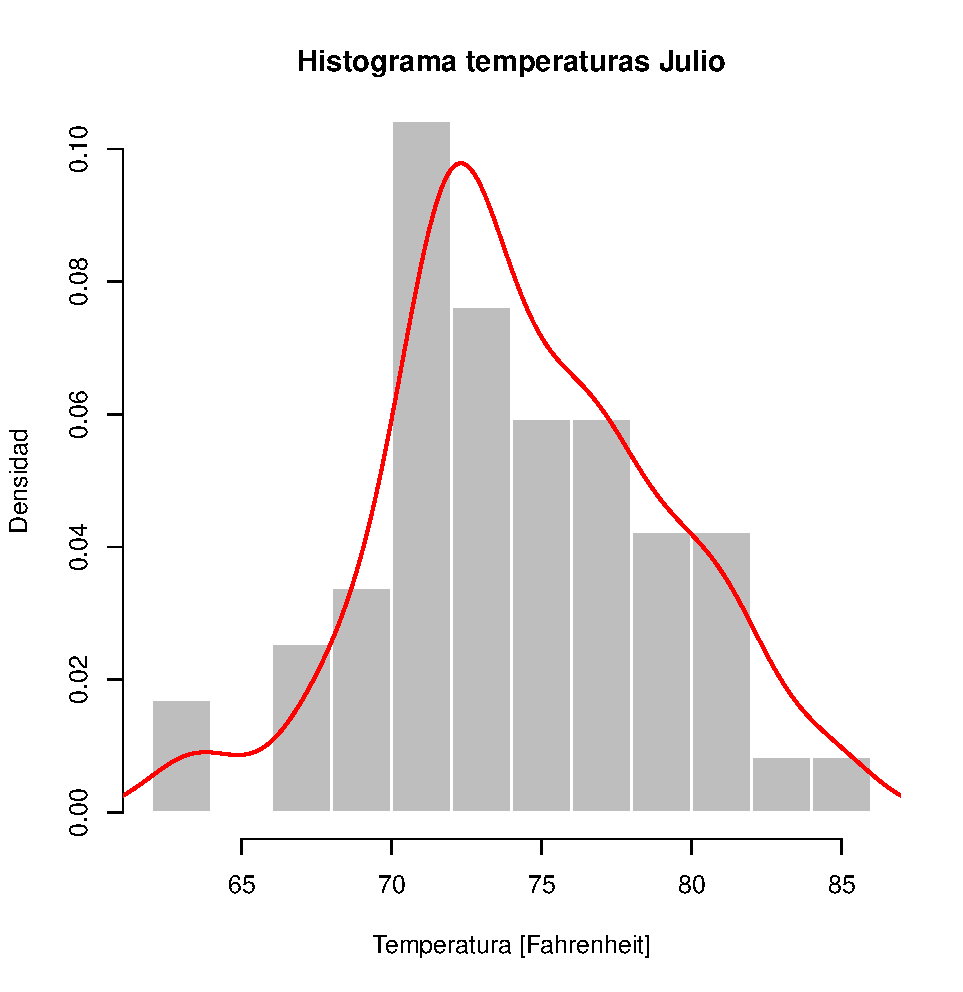
\includegraphics[scale = 0.3]{histtj}
    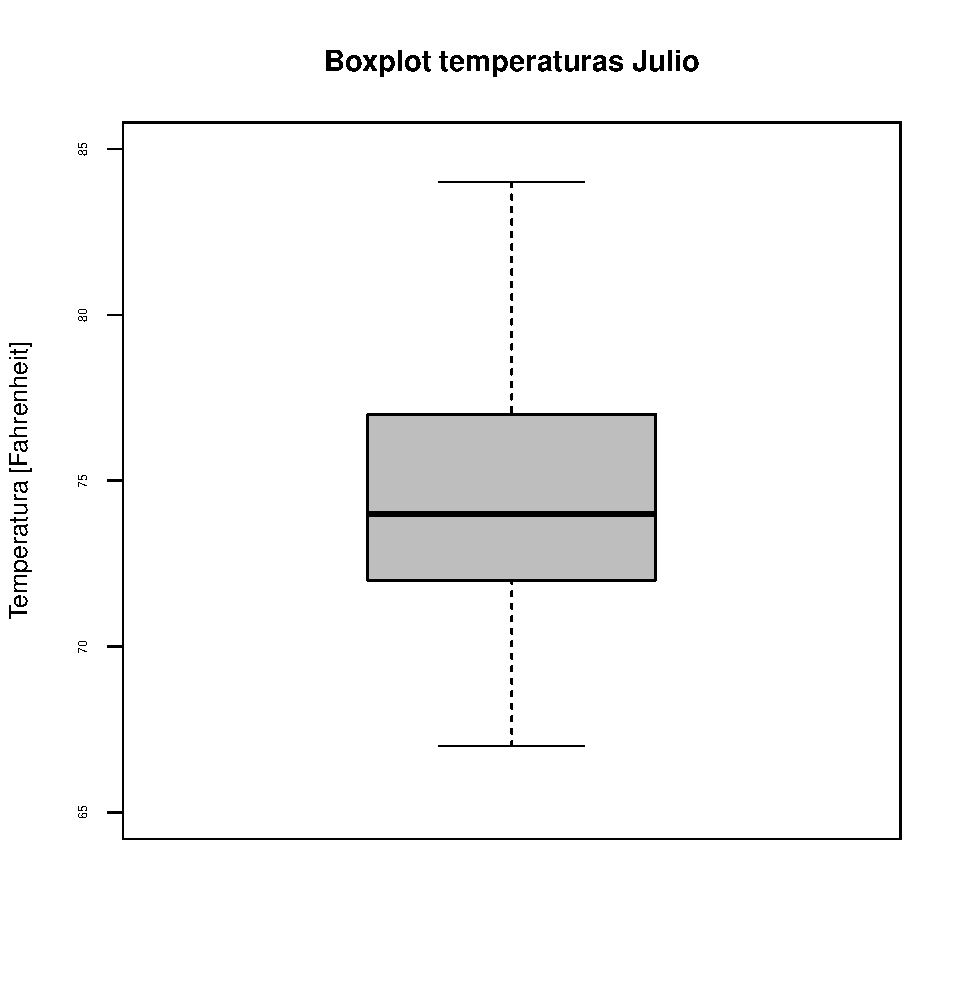
\includegraphics[scale = 0.3]{boxtj}
\end{center}

Si bien el histograma está cargado al medio, no tenía tanta simetría como esperábamos. El boxplot es bastante simétrico con una pequeña tendencia a la baja.

\section{Mortalidad y gases contaminantes}

Los gases contaminantes descritos al principio del informe podrían tener cierta relación con la mortalidad de la zona. Para estudiar esto, analizaremos gráficos de mortalidad vs.  presencia del gas 

\subsection{NOx}

\textbf{Gráfico Mortalidad vs. Presencia de NOx:}

\begin{center}
    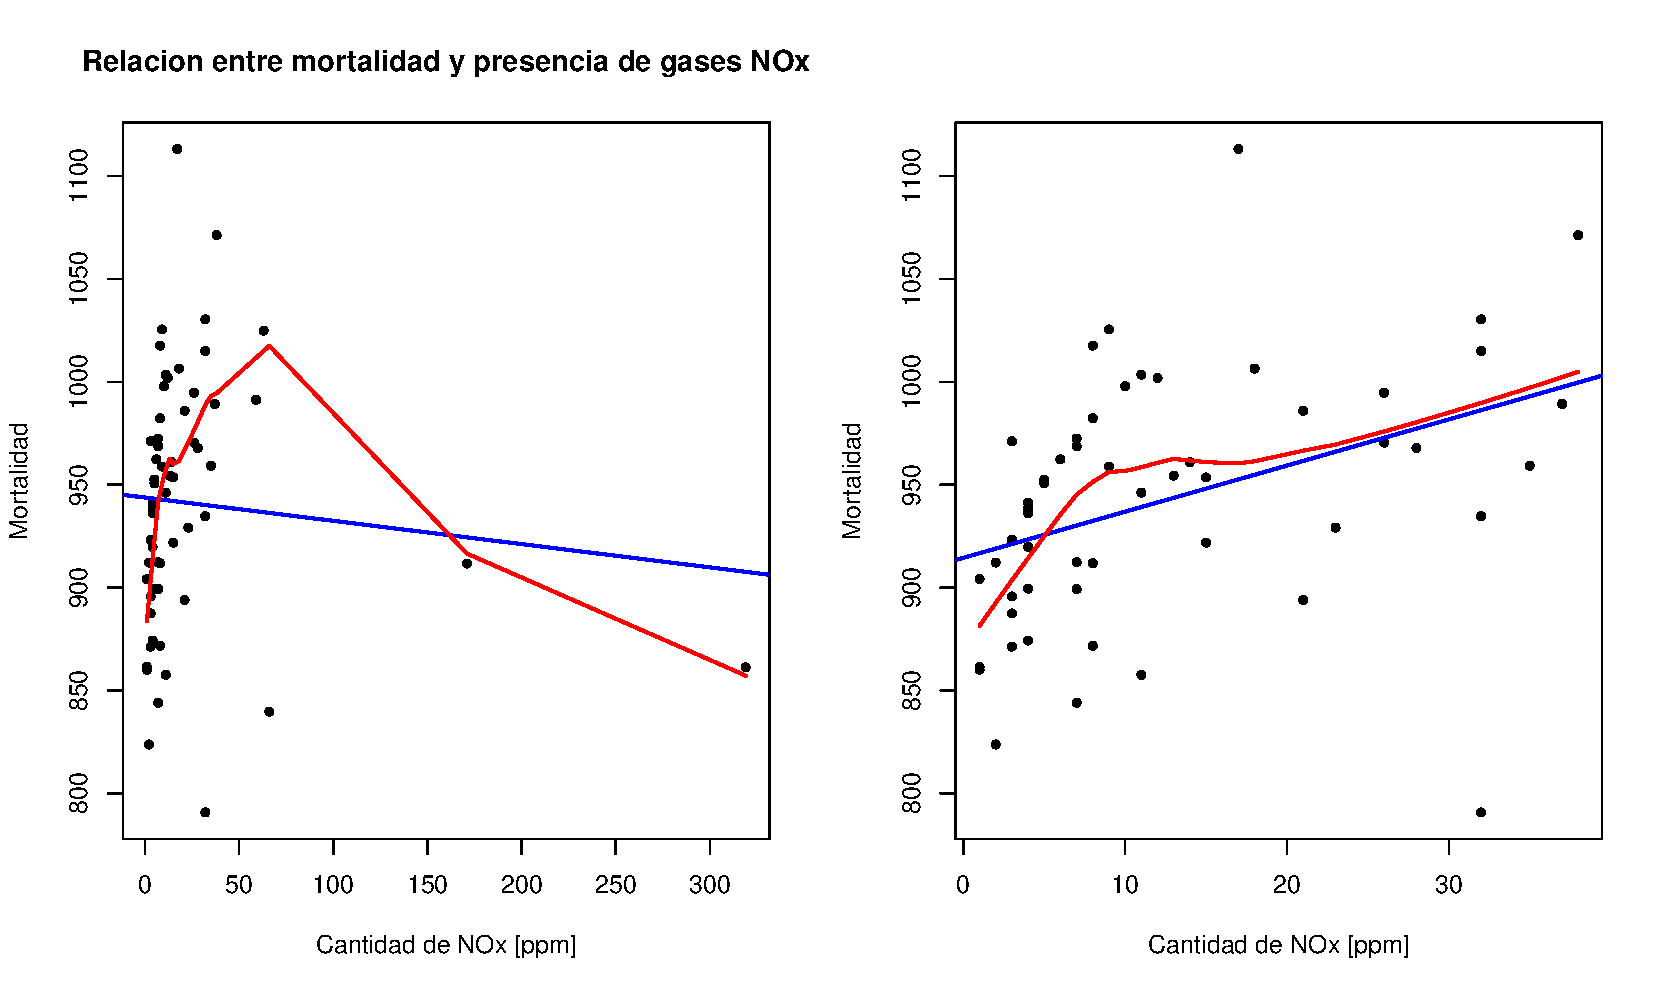
\includegraphics[scale = 0.4]{mortnox}
\end{center}

En estos gráficos las lineas rojas y azules ajustan la relación entre los puntos, las primeras con una función aproximada y las segundas con una regresión lineal.

Observamos dos gráficos, el primero es la relación entre todos los valores de NOx y la mortalidad, este nos entrega una relación inversa entre las variables. Esto no es esperado porque NOx es dañino para la salud, el problema es que, como vimos en la sección anterior, la variable de NOx tiene outliers que no deben ser considerados ya que no representan conclusiones estadísticas sólidas. Si acotamos la cantidad de NOx a 40[ppm] obtenemos el segundo gráfico. En este, como vimos antes, si existen suficientes datos como para hacer conclusiones. Deducimos entonces que a mayor cantidad de NOx efectivamente, aumenta la mortalidad.

La pendiente de la segunda recta es de aproximadamente 2.2, lo que significa un aumento en la mortalidad de 2.2 por cada [ppm] de NOx adicional.

La acotación anterior debe hacerse puesto que la mortalidad depende de muchas variables, y para relacionarla con alguna de estas debemos obtener una tendencia que se sostenga en varios casos.

\subsection{HC}

\textbf{Gráfico Mortalidad vs. Presencia de HC:}

\begin{center}
    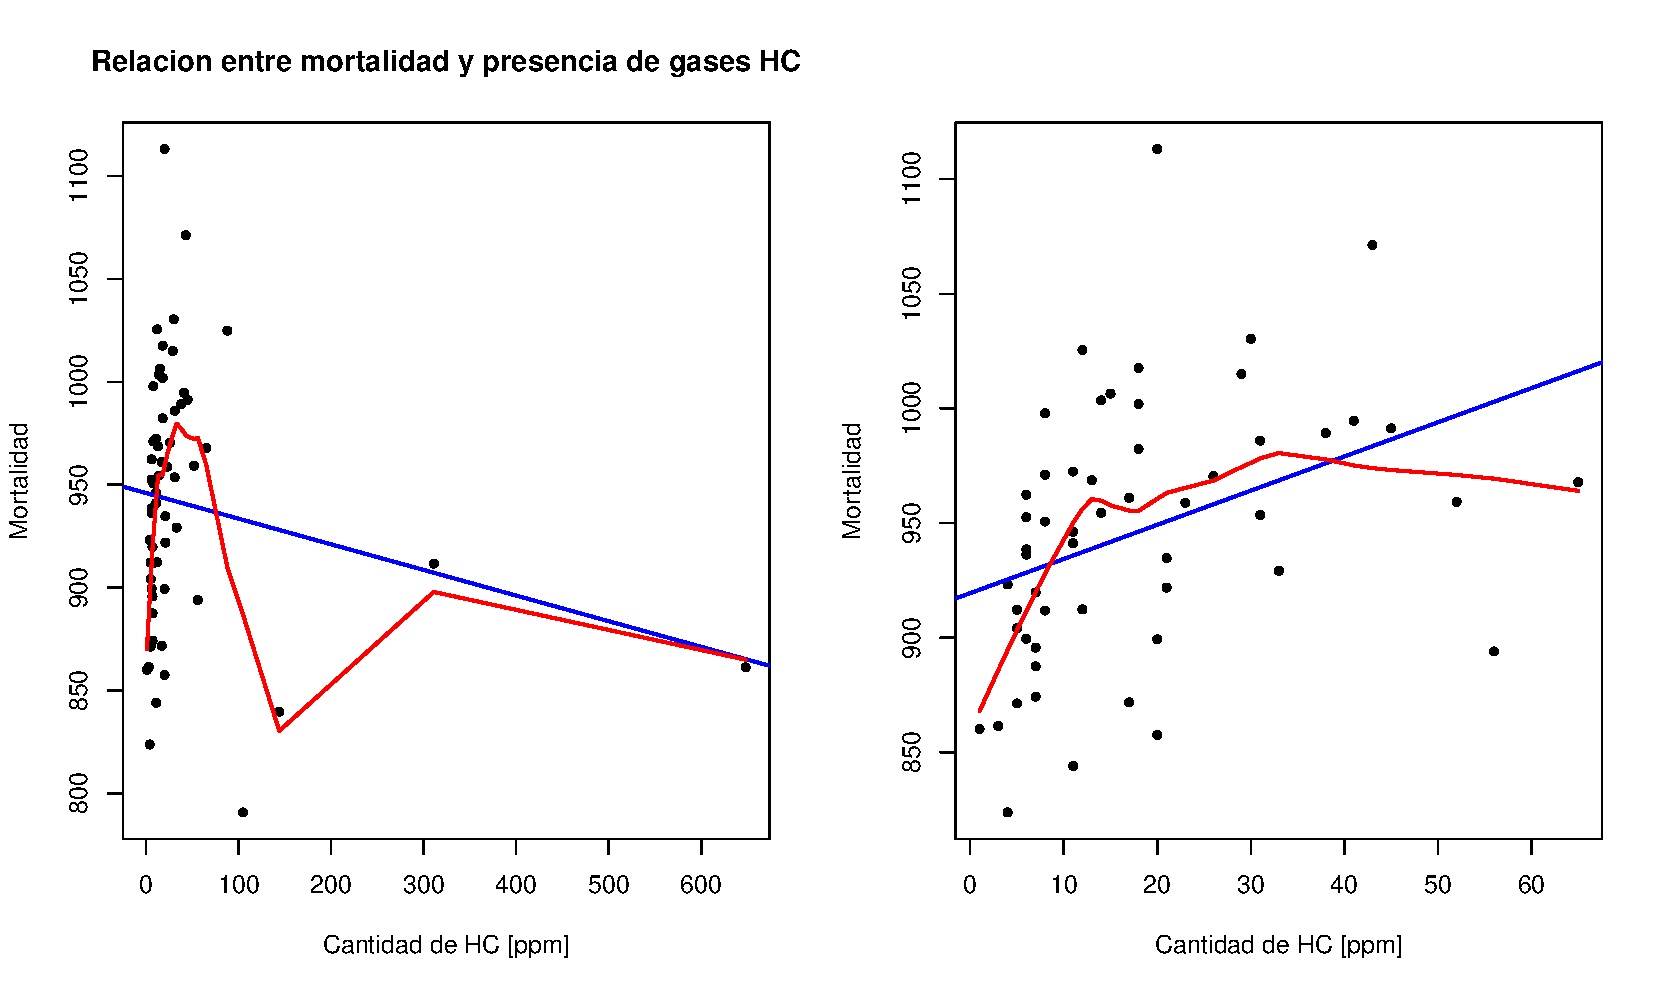
\includegraphics[scale = 0.4]{morthc}
\end{center}

Al igual que en NOx, los outliers alteran el gráfico si tomamos todos los valores de HC, pero si tomamos hasta 70[ppm] que es, como vimos en la sección 2.1.2, donde se concentra la mayor cantidad de datos, obtenemos de nuevo que a mayor presencia de HC aumenta la mortalidad.

La pendiente de la segunda recta es de aproximadamente 1.5, lo que significa un aumento en la mortalidad de 1.5 por cada [ppm] de HC adicional.

\subsection{SO_2$}

\textbf{Gráfico Mortalidad vs. Presencia de SO_2:$}

\begin{center}
    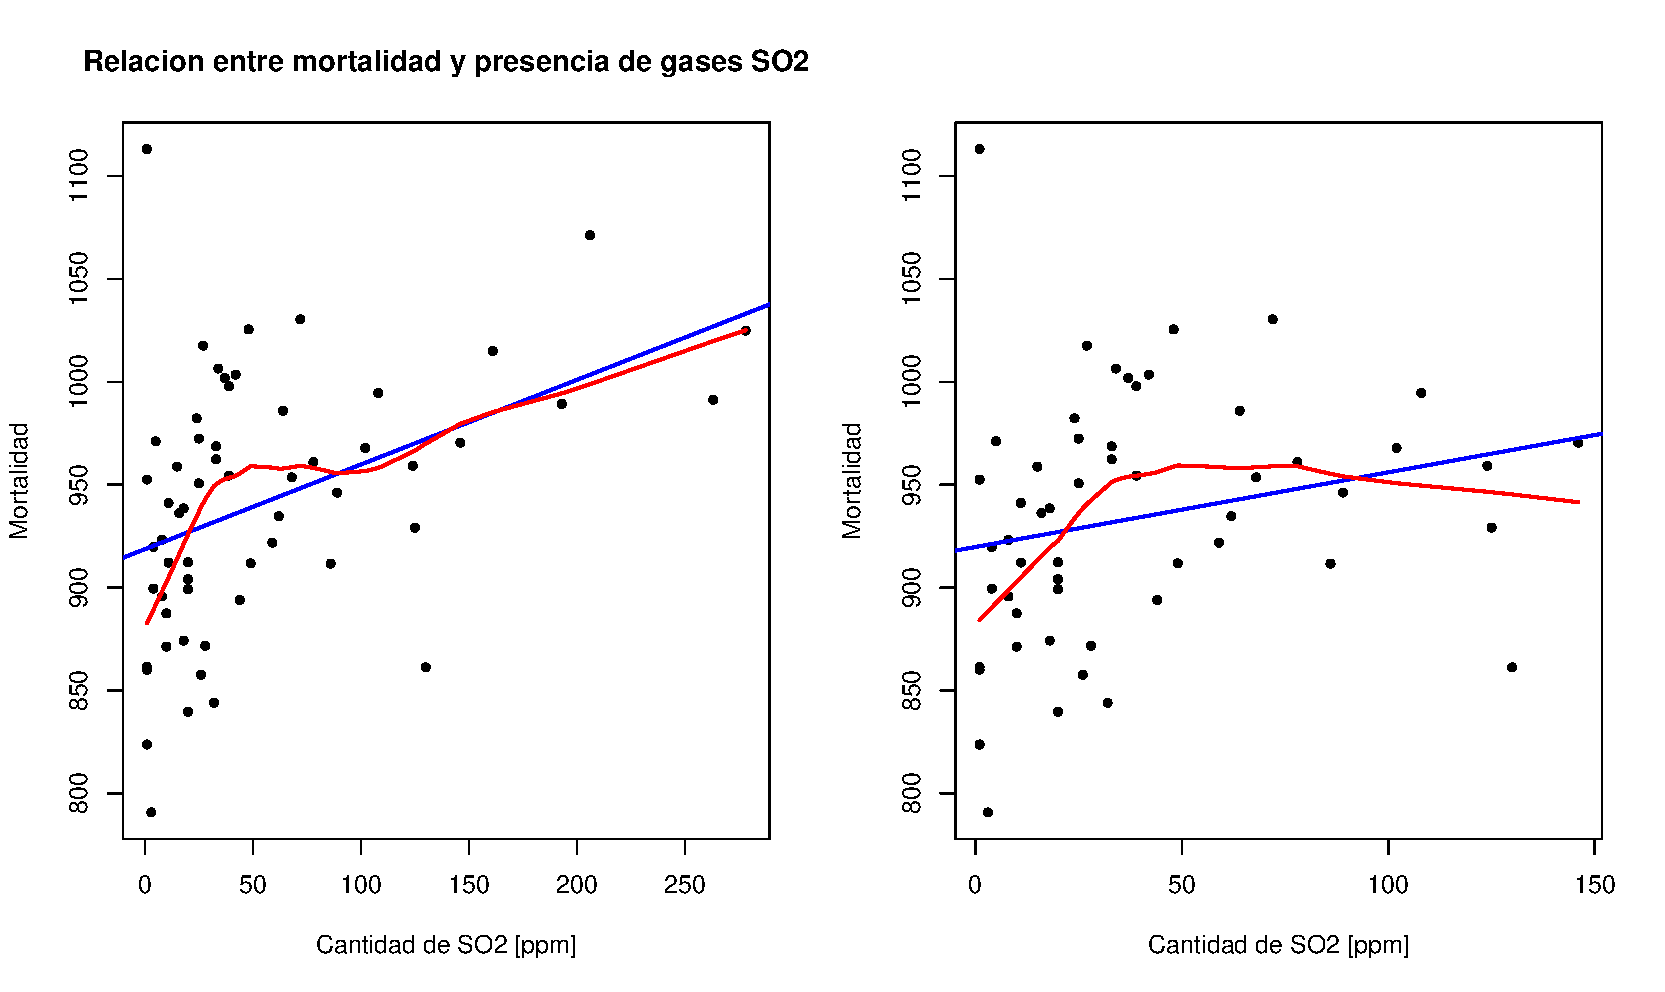
\includegraphics[scale = 0.4]{mortso2}
\end{center}

Con el SO_2$ no encontramos el problema de antes, aun con todos los datos este gas presenta una relación de proporcionalidad directa con la mortalidad, de todas maneras graficamos la zona de alta densidad obtenida en 2.1.3 para confirmar nuestro resultado.

La pendiente de las rectas es aproximadamente 0.35, lo que significa un aumento de la mortalidad en 0.35 por cada [ppm] de SO_2$ que aumenta en el ambiente.

\subsection{Conclusión}

Los tres gases presentan un efecto agravante en la mortalidad de la población, siendo NOx que tiene la mayor tasa de aumento de mortalidad por cada [ppm] adicional, y SO_2$ el con menor tasa de aumento.

\section{Contaminación en NY y OH}

Podemos comparar la contaminación entre ambos estados, a continuación se presentan gráficos de cajas para cada gas lado a lado (con la misma escala para que sea más fácil comprarar visualmente):

\begin{center}
    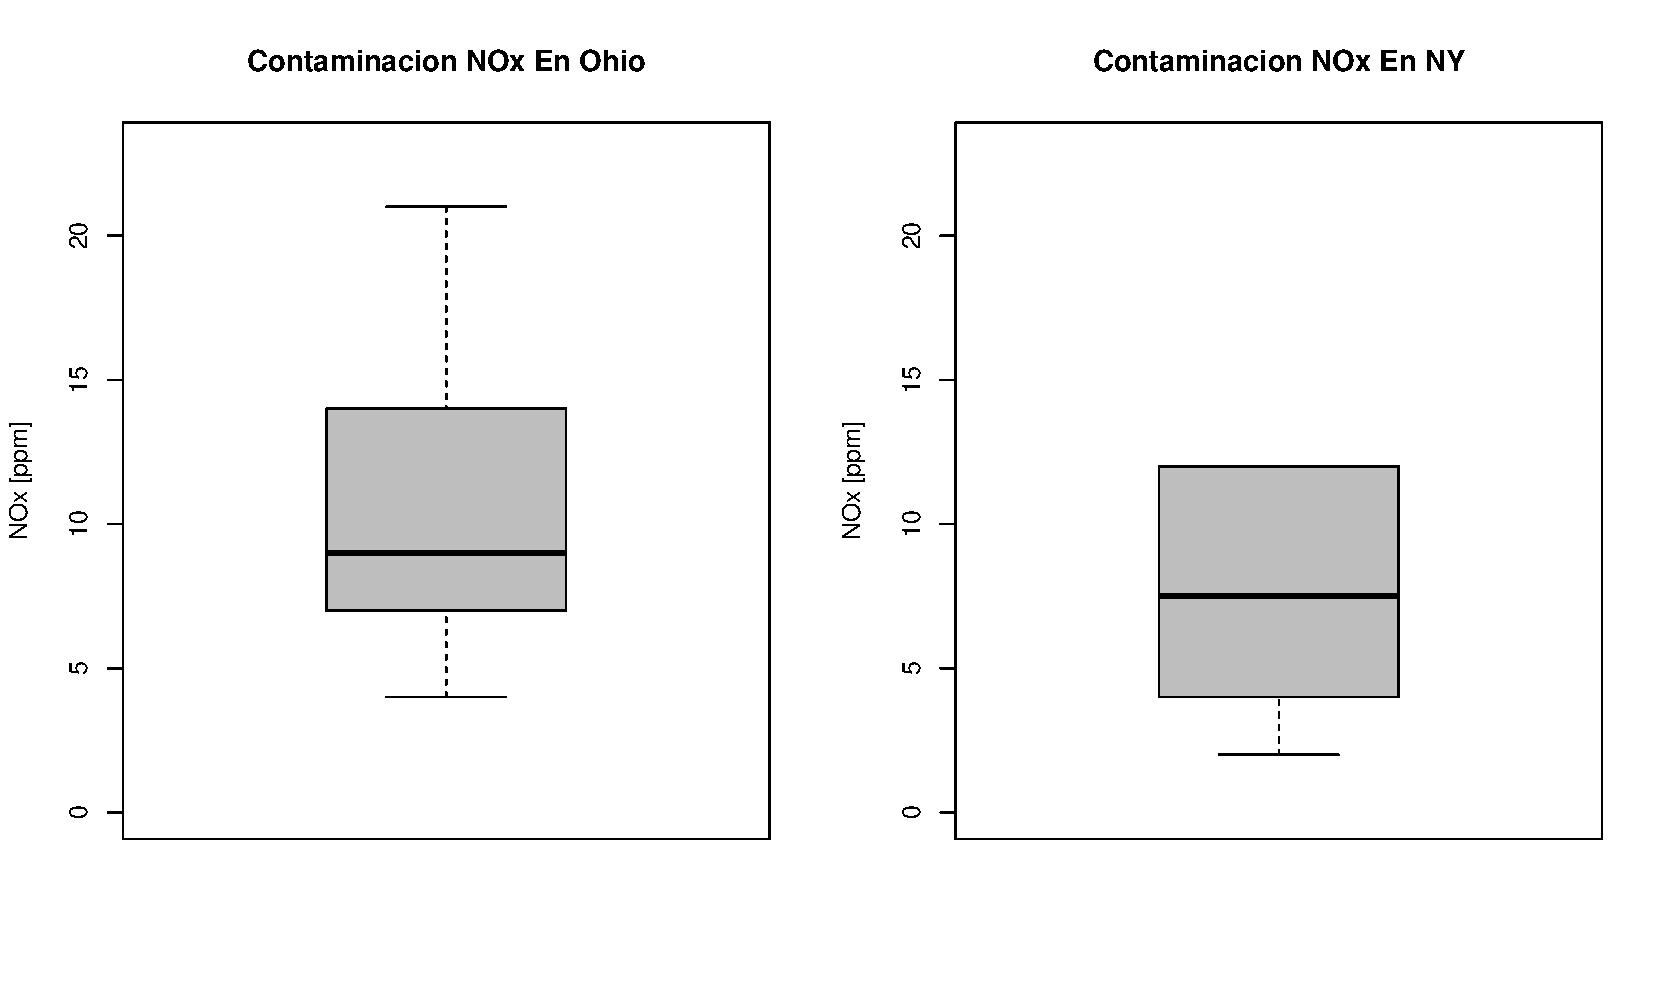
\includegraphics[scale = 0.4]{ohnynox}
    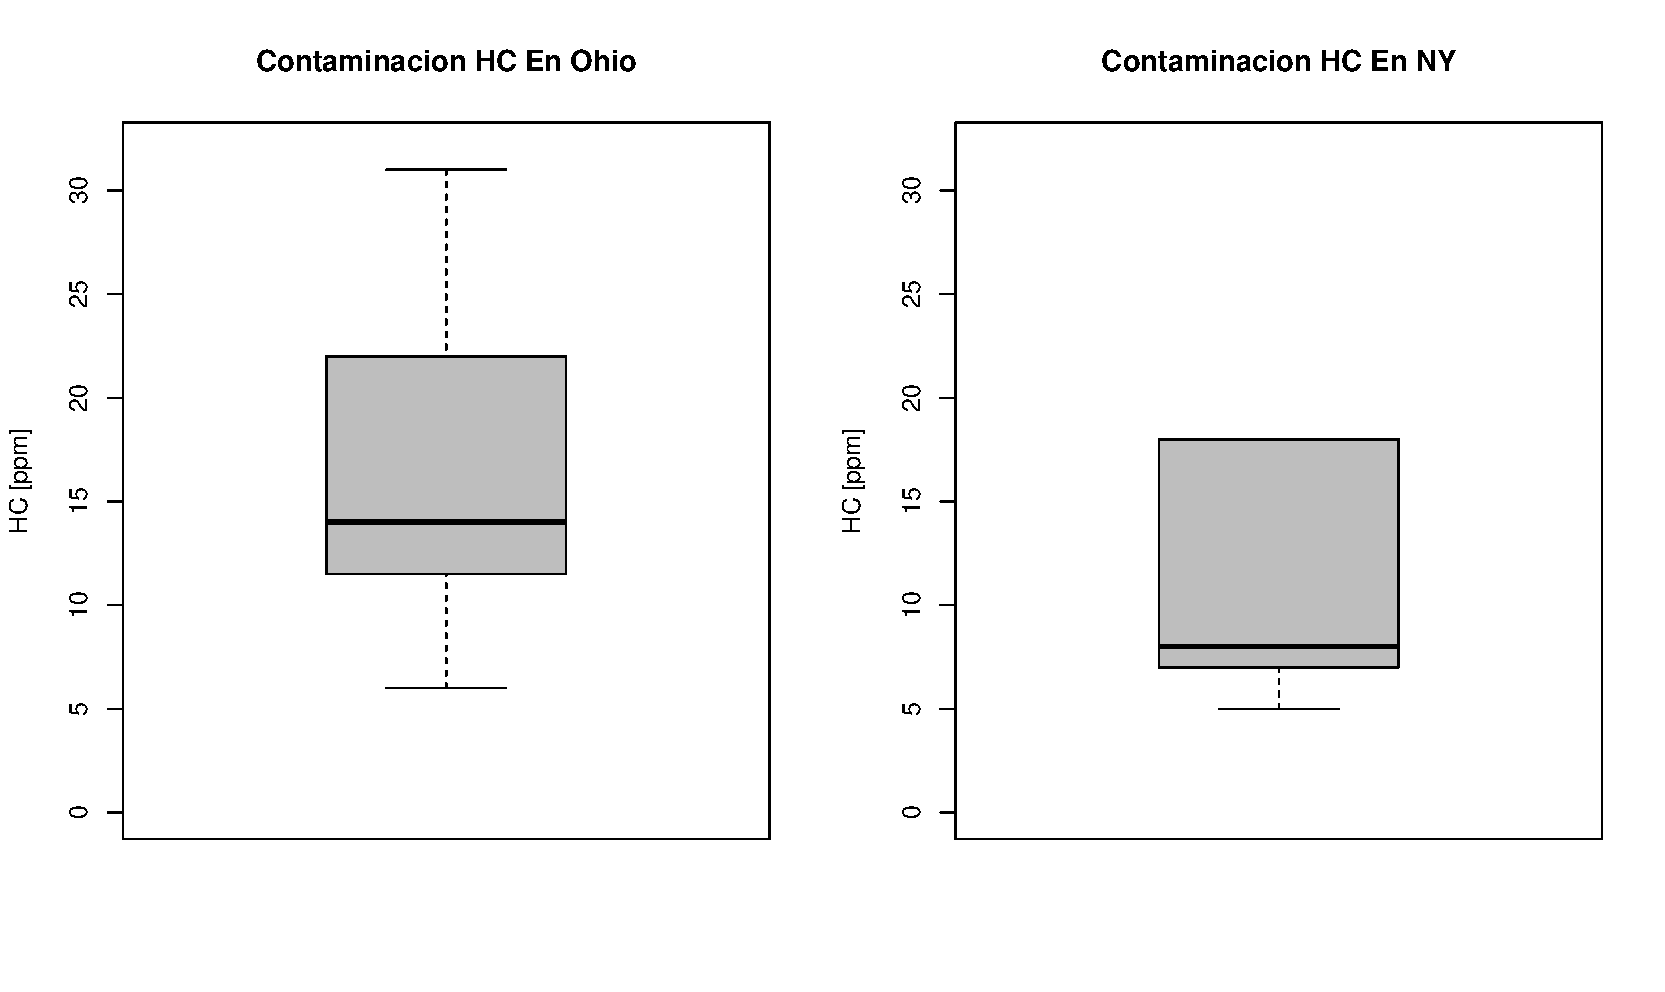
\includegraphics[scale = 0.4]{ohnyhc}
    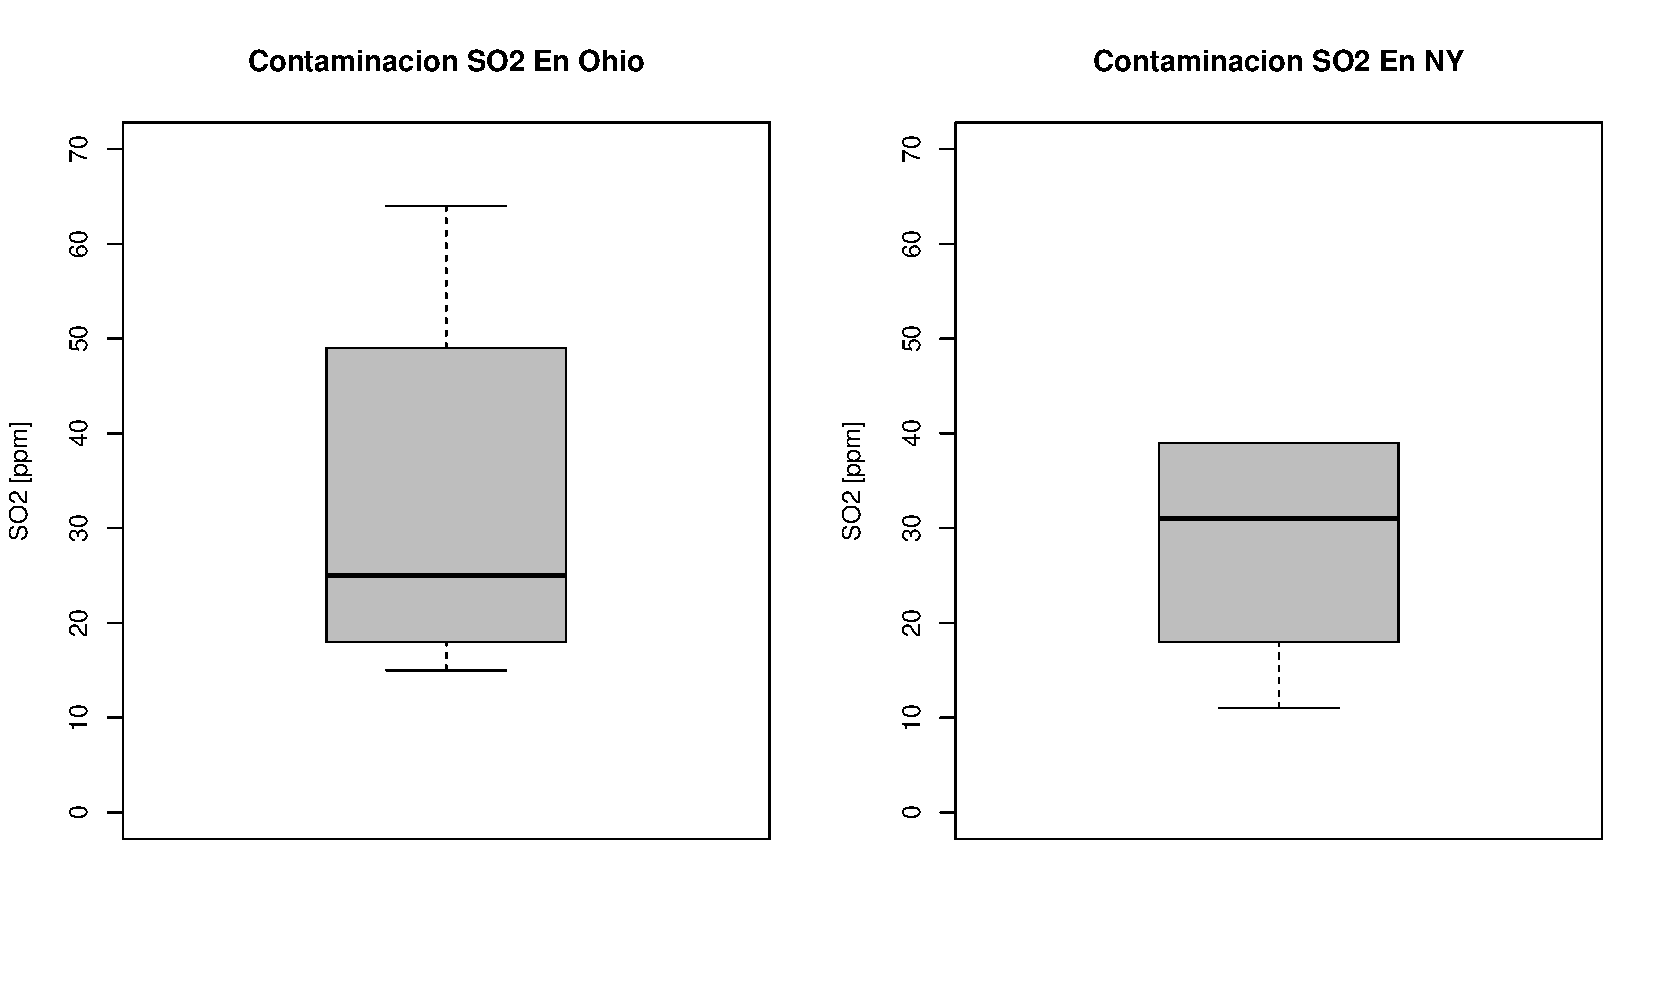
\includegraphics[scale = 0.4]{ohnyso2}
\end{center}

Notamos como Ohio, para los tres gases, tiende a presentar valores mayores de contaminación

\section{Ajuste de modelo para población por hogar}

Por último, buscamos ajustar un modelo de probabilidad a la variable de población por hogar estudiada en la sección 2.2.2, recordamos su histograma de distribución:

\begin{center}
    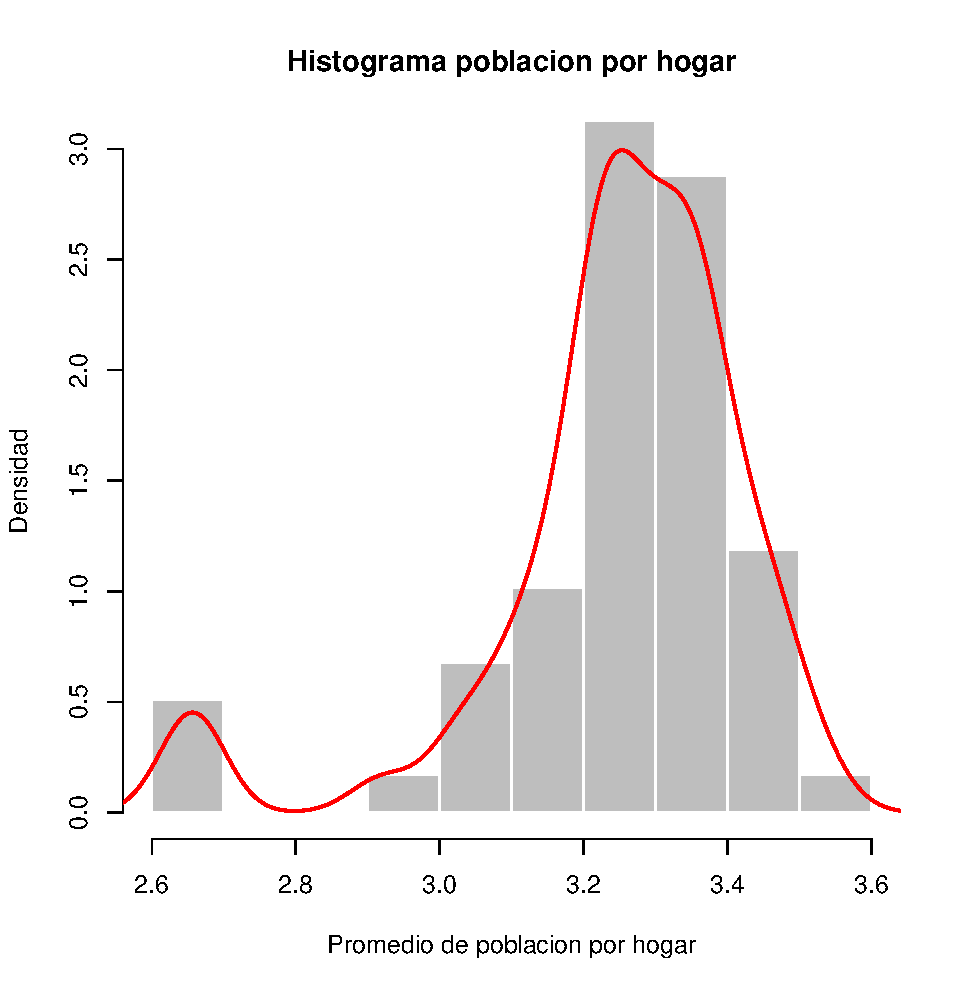
\includegraphics[scale = 0.5]{histph}
\end{center}

Buscamos un modelo en la familia de localización y escala, o sea alguno de:

\begin{itemize}
    \item Distribución Exponencial trasladada
    \item Distribución Normal
    \item Distribución Logística
\end{itemize}

Recordando que los modelos de localización y escala son aquellos que tienen un parametro de escala no negativo y uno de localización.

Para hacer esto ordenamos la variable de forma creciente con respecto a su probabilidad, hacemos una regresión lineal para intentar alinearla con la función de distribución y podemos analizar gráficamente qué modelo se adapta mejor, siendo este cuya recta se acerque más al gráfico de los valores.

\begin{center}
    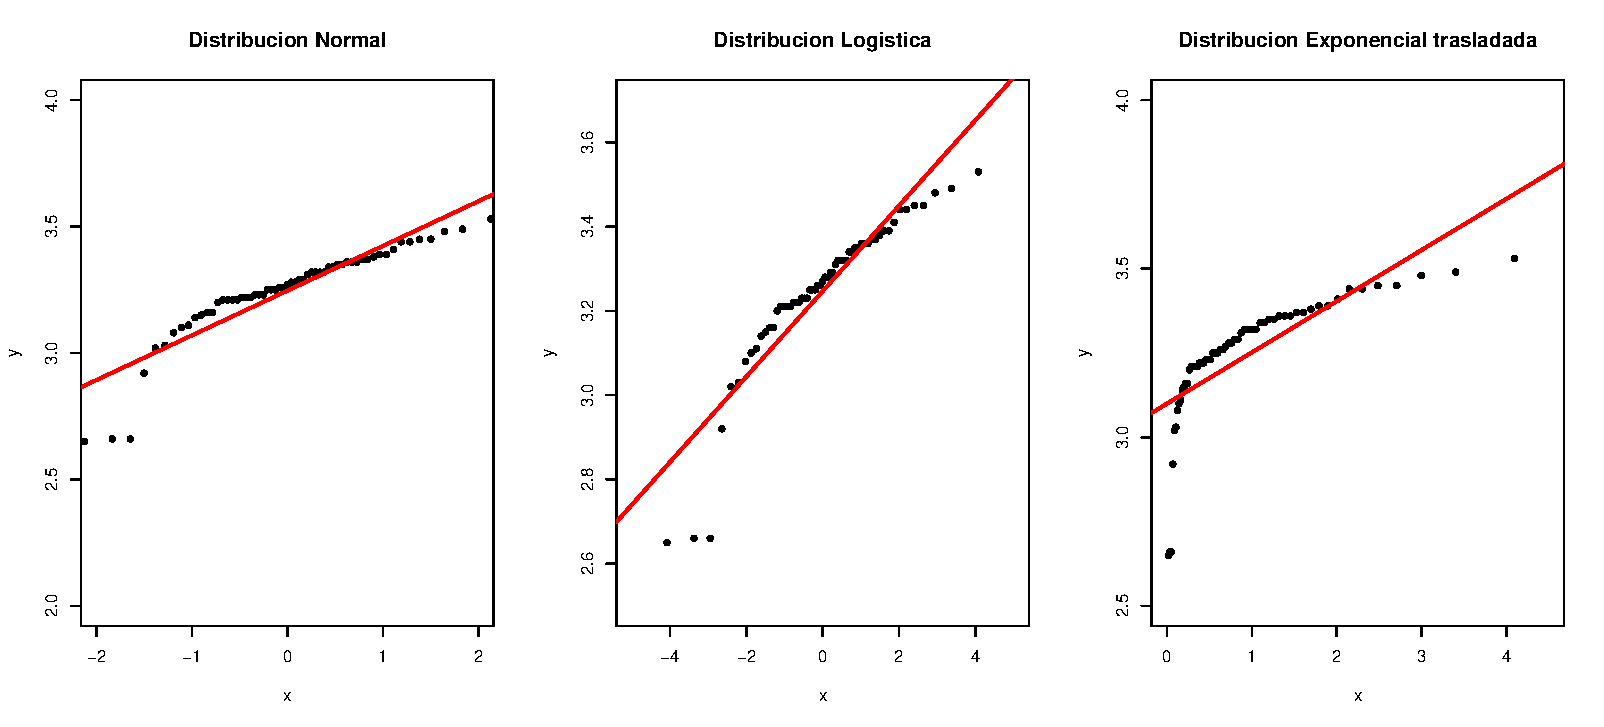
\includegraphics[scale = 0.5]{modelchoose}
\end{center}

Notamos que, la recta más ajustada es la de la distribución logística, seguido de cerca por la normal. Podemos confirmar esto con el gráfico de densidad y los tres modelos:

\begin{center}
    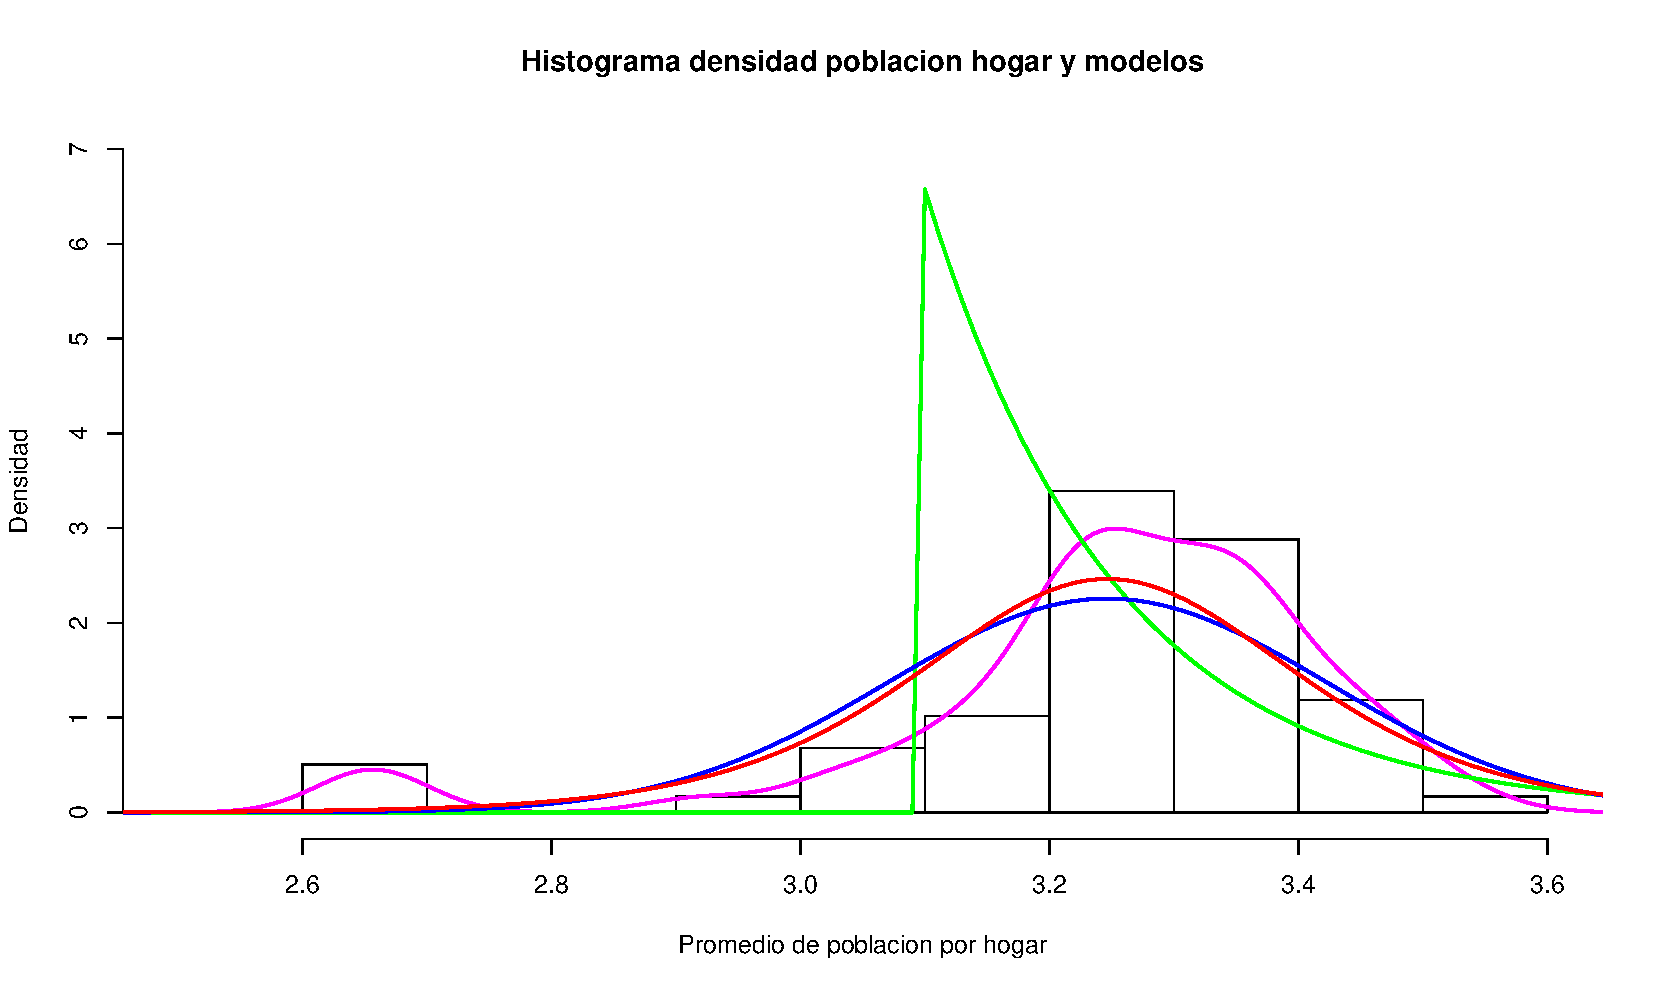
\includegraphics[scale = 0.5]{modelfit}
\end{center}

Donde la línea magenta representa la densidad de la variable, la roja es la distribución logística, la azul la normal y la verde la exponencial trasladada.

Se concluye entonces que:

\begin{center}
    Población por hogar \sim$ Logística(3.25, 0.1)
\end{center}

\end{document}
